%-----------------------------------------------%
%---------------------------------------------%
%
% BACHELOR OF SCIENCE THESIS
%
% Emanuele Ballarin <emanuele@ballarin.cc>
%
% Prof. Luca Bortolussi, Prof. Fabio Benatti
%
%---------------------------------------------%
%
% Bachelor's Degree in Physics
%
% Dept. of Physics
% University of Trieste, Italy
%
% 24-27/04/2020
%
% A.Y. 2018/2019
%
%---------------------------------------------%
%-----------------------------------------------%


% Document configuration %
%---------------------------------------------%
\documentclass[a4paper, twoside]{article}
%---------------------------------------------%

% Used packages and configuration %
%------------------------------------------------------------------------%
\usepackage[utf8]{inputenc}
\usepackage{natbib}
\usepackage{graphicx}
\usepackage{amsmath}
\usepackage{mathtools}
\usepackage{wrapfig}
\usepackage{amsfonts}
\usepackage{csquotes}
\usepackage{float}
\usepackage{graphicx,wrapfig,lipsum}
\usepackage{blindtext}
\usepackage{multirow}

% MARGINS %
\usepackage{geometry}\geometry{top=2.5cm,bottom=2.5cm,left=3cm,right=3cm} % symmetric
%\geometry{top=2cm,bottom=2cm,right=3cm,left=1.8cm,headheight=15pt}   % A-symmetric

\usepackage{fancyhdr}
\usepackage{bm}
\usepackage{xcolor}
\usepackage[titletoc]{appendix}
\usepackage{upgreek}

% FANCYHDR CONFIG %
\pagestyle{fancy}
\fancyhead{}
\renewcommand{\headrulewidth}{0.4pt}
\renewcommand{\footrulewidth}{0.4pt}
\setcounter{secnumdepth}{4}

% CHAPTER TITLES CONFIG %
\usepackage{titlesec}
\titleformat{\chapter}[display]{\normalfont\Huge\bfseries}{\chaptertitlename\ \thechapter}{15pt}{\Huge}
\titlespacing*{\chapter}{0pt}{-3\baselineskip}{20pt}[3.7cm]% Moves the chapter title out of the text block. Do you really want this?
\assignpagestyle{\chapter}{empty}

\usepackage{nomentbl}
\usepackage{enumitem,calc}
\usepackage{lscape}
\usepackage{setspace}\linespread{1.4}
\usepackage{parskip}
%------------------------------------------------------------------------%


% Document declaration %
%------------------------------------------------------------------------%
\begin{document}
\begin{titlepage}
\newcommand{\HRule}{\rule{\linewidth}{0.5mm}} % Defines a new command for the horizontal lines, change thickness here
\center % Center everything on the page (why unrecognized??)
%------------------------------------------------------------------------%


% HEADINGS %
%------------------------------------------------------------------------%
\vspace{-16mm}
\vspace*{16mm}
\textsc{\LARGE{Università degli Studi di Trieste}}\\[1.5cm] % Name of your university/college
%------------------------------------------------------------------------%


% LOGO %
%------------------------------------------------------------------------%

\includegraphics[width=0.30\linewidth]{logouniv.png} % Include a department/university logo - this will require the graphicx package
%------------------------------------------------------------------------%


% TITLES %
%------------------------------------------------------------------------%
\HRule \\[0.4cm]
{ \huge \bfseries Modelli generativi di modelli neurali artificiali robusti}\\[0.4cm] % Title of your document
{ \LARGE Uno studio preliminare di fattibilità}\\[0.4cm]
\HRule \\[1.5cm]
%------------------------------------------------------------------------%


% AUTHOR %
%------------------------------------------------------------------------%
\begin{minipage}{0.4\textwidth}
\begin{flushleft}
\Large \emph{{Autore:}}\\
{Emanuele} \textsc{{Ballarin}} % Your name
\end{flushleft}
\end{minipage}
~
\begin{minipage}{0.4\textwidth}
\begin{flushleft}
\Large \emph{{Relatore:}} \\
{Prof. Luca}  \textsc{{Bortolussi}} \\ % Supervisor's Name

\emph{{\\ Co-Relatore:}} \\
{Prof. Fabio}  \textsc{{Benatti}}
\end{flushleft}
\end{minipage}\\[2cm]
%------------------------------------------------------------------------%


% DATE and PLACE %
%------------------------------------------------------------------------%
\Large
\textsc{Dipartimento di Fisica\\
A.A. 2018/2019}
\vfill % Fill the rest of the page with whitespace
\end{titlepage}
%------------------------------------------------------------------------%


% LEADING EMPTY PAGE and T.O.C. %
%------------------------------------------------------------------------%
\newcommand{\blankpage}{
	\newpage
	\thispagestyle{empty}
	\mbox{}
	\newpage}

\blankpage
\newpage
\renewcommand{\contentsname}{Indice}  % Easy language compatibility (no additional package)
\setcounter{section}{-1}			  % Index section starts from 0
\tableofcontents
%------------------------------------------------------------------------%


% ABSTRACT %
%------------------------------------------------------------------------%
\newpage
\section{Abstract}

Il presente lavoro di tesi, redatto in osservanza dei requisiti per il conferimento del titolo di \textit{Laurea in Fisica} (triennale), si occupa di formulare, esplorare e valutare preliminarmente un nuovo approccio originale per il \textit{training} di modelli basati su reti neurali profonde (\textit{Deep Learning}), che siano in grado di soddisfare opportune proprietà di \textit{adversarial robustness} -- ovverosia di resistenza a perturbazioni degli input, costruite ad arte con il fine di produrre un comportamento non corretto (o non previsto) nei modelli suddetti -- senza sacrificare accuratezza, o facendolo al più in modo controllabile.

In particolare, l'approccio proposto mira a raggiungere suddetti obiettivi attraverso la generazione dei \textit{pesi} della rete neurale in analisi tramite un modello generativo e un \textit{value network} ausiliario che ne determina la \textit{funzione costo}, entrambi a loro volta reti neurali profonde. Questa modalità di procedere si distingue, da quella attualmente più seguita per il medesimo scopo (e con risultati sicuramente lontani dall'essere definitivi), nel non ricorrere alla \textit{backpropagation} direttamente sul modello in analisi come strategia per produrre \textit{robustezza}.

Dopo aver contestualizzato il paradigma contemporaneo del \textit{Deep Learning} all'interno dei più generali ambiti dell'\textit{Intelligenza Artificiale} e del \textit{Machine Learning}, il presente elaborato fornisce un'introduzione ai suoi elementi caratterizzanti e fondativi, ad alcune tecniche collegate -- in uso nel seguito --, e al problema dell'\textit{adversarial robustness} per i modelli così prodotti.\\
Successivamente, sono proposte una misura di \textit{adversarial robustness globale} e una metrica che tenga esplicitamente conto di un eventuale \textit{tradeoff} tra accuratezza e \textit{robustezza}. Dunque, facendone uso, è dettagliato l'approccio originale proposto e sono altresì descritte le procedure sperimentali che si sono seguite al fine di verificarne il buon comportamento.

Da ultimo, sono riportate le conclusioni maturate grazie a tale esperienza, gli aspetti di maggior validità e di eventuale criticità dell'approccio proposto, e le prospettive di ricerca futura che da esso vengono offerte e suggerite per il futuro.



% INTRODUCTION %
%------------------------------------------------------------------------%
\newpage
\section{Introduzione}

Sin dalle sue origini, e in misura ben più marcata a partire dalla \textit{Prima Rivoluzione Industriale}, lo sviluppo della civiltà umana è stato caratterizzato dalla realizzazione di strumenti -- di crescente efficacia, efficienza e varietà d'applicazioni -- che potessero migliorare la condizione dei suoi membri e massimizzare la capacità di soddisfacimento dei più disparati bisogni.

Tuttavia, pur in seguito all'avvento delle tecnologie informatiche di massa e sicuramente fino agli anni 10 del secolo in corso, tale tentativo in contesto \textit{di produzione} non si è mai concretizzato nell'automazione di funzioni cognitive di ordine superiore -- quand'anche animali, se non umane -- come il \textit{ragionamento deduttivo}, l'\textit{inferenza induttiva e causale}, l'\textit{elaborazione delle informazioni sensoriali} (\textit{visione} prima fra tutte), la \textit{capacità decisionale}.

Il tentativo, tuttavia, di affrontare in modo rigoroso e quantitativo il problema del \textit{funzionamento della mente}, dell'apprendimento e della cognizione -- con il fine derivarne un modello ed, eventualmente, simularlo artificialmente -- può essere già trovato nei lavori di McCulloch \& Pitts (1943), Hebb (1949), Minsky \& Papert (1969) e Hopfield (1980).\\
In particolare, tali approcci si distinguono dal pur popolare (all'epoca come oggi) filone della \textit{logica} (anche computazionale) e dei sistemi di deduzione automatica -- con finalità parzialmente sovrapposte -- per il loro carattere estremamente generale, non orientato alla specifica attività da svolgere, e fondato essenzialmente sulla formalizzazione e modellazione matematica del funzionamento dei neuroni e delle loro interconnessioni, in forma approssimata.

Tale dicotomia metodologica (non priva tuttavia di reciproche influenze e commistioni) ha portato tradizionalmente a suddividere il vastissimo ambito di ricerca della cosiddetta \textit{Intelligenza Artificiale} -- altresì detta \textit{Intelligenza Computazionale} -- nel filone \textit{simbolico} (il secondo, orientato principalmente alla manipolazione di simboli e predicati con finalità deduttive) e quello \textit{connessionista} (il primo, ispirato al funzionamento degli aggregati di neuroni biologici \textit{lato sensu}, e oggi talvolta citato, senza una chiara convenzione sull'uso dei termini, anche con i nomi di \textit{cognitive computing} o \textit{neuroscienze matematiche/computazionali}).

Per ciascuno di questi due approcci alla ricerca \textit{fondamentale}, nel corso degli ultimi cinquant'anni, sono state sempre più spesso proposte eventuali applicazioni industriali e commerciali, con una discreta dominanza del filone \textit{simbolico} negli anni '80 e '90, per poi assistere ad una ripresa di popolarità del \textit{connessionismo} culminata (o meglio, culminante tutt'oggi) con la \textit{Deep Learning revolution} iniziata durante lo scorso decennio.

L'influente e più che ventennale lavoro dei gruppi di ricerca guidati Hinton, LeCun e Bengio -- proprio per questo insigniti dell'\textit{ACM Turing Prize} nel 2008 --, l'accesso a sempre più potenti e meno costosi calcolatori equipaggiati con \textit{hardware} di consumo adatto ai calcoli richiesti da questo particolare tipo di approccio (come le \textit{GPU} parte delle schede grafiche dedicate) e il crescente interesse e finanziamento in tale direzione da parte di soggetti privati, interessati alle applicazioni commerciali del paradigma, sono considerati i fattori di maggiore rilevanza per spiegare tale popolarità senza precedenti. La necessità di una notevole quantità di dati per garantire il corretto \textit{training} dei modelli neurali profondi -- congiunta a un periodo come quello attuale in cui connettività a Internet diffusa, dispositivi \textit{smart} per uso personale e il cosiddetto \textit{Internet of Things} possono proprio contribuire alla loro raccolta -- spiega infine le ragioni del successo commerciale di questa tecnologia.

All'attuale \textit{stato dell'arte}, il \textit{Deep Learning} si dimostra il più ricco ed espressivo \textit{framework} noto di \textit{modellazione statistico-probabilistica}, capace di successi talvolta conosciuti anche dal grande pubblico. Da segmentazione e riconoscimento d'immagini (e pure facciale), al riconoscimento vocale, alla diagnosi clinica \textit{computer-aided} quando non completamente automatica, alla classificazione, traduzione e addirittura scrittura \textit{ex-novo} di testi, documenti e \textit{corpora} letterari, alla guida autonoma di autoveicoli in ambiente controllato, a un'automazione industriale dotata di un'\textit{intelligenza} più simile a quella \textit{umana}.


%------------------------------------------------------------------------%


\newpage
\section{The Neural Network Paradigm}

An artificial neural network (ANN) is, rather than an algorithm, a framework for which an \textit{architecture} and a \textit{learning rule} are defined. Within this framework, given a dataset, it is possible to find an algorithm which correctly makes predictions on that data, to extract information on the input distribution, or to efficiently reduce the input dimensionality by preserving its \textit{information}.

During their first decades, a strong connection between neural networks and statistical physics was established. However, in the last fifteen years neural networks have become \textit{deep}, as we will discuss in Chapter 4, with a huge increase in the number of parameters and complexity. As a consequence, the common ground between statistical mechanics and modern neural networks, which are properly called \textit{deep neural networks}, is difficult to analyze.

Although it won't be the focus of this thesis, we want to briefly introduce the framework in which neural networks were studied in their first years, so that the reader will be able to grasp the modern techniques we will introduce in the following chapters with a broader perspective.

    \subsection{Perceptron and separability}

    In 1958, Frank Rosenblatt introduced the first linear model which was able to learn its parameters: the very prototype of today's supervised learning models. Such a neural model consists of a linear combiner followed by a \textit{hard limiter}. Inputs are applied to the synapses, an affine combination is performed, and ultimately the signum function is applied. We define $w$ as the synapses' intensities vector, $x$ the input vector, and $y$ the output scalar. The transformation performed on $\boldsymbol{x}$ is:

    $$ y = \text{sgn}\left( \sum_{i=1}^m x_i w_i \quad + b \right)$$

    The learning rule for this model is:

    $$ \boldsymbol{w} \rightarrow \boldsymbol{w'} = \boldsymbol{w} + \epsilon (\xi - y) \boldsymbol{x}$$

    where $\xi$ is the desired output, i.e. the correct answer for the given input.


    \begin{figure}[H]
        \centering
        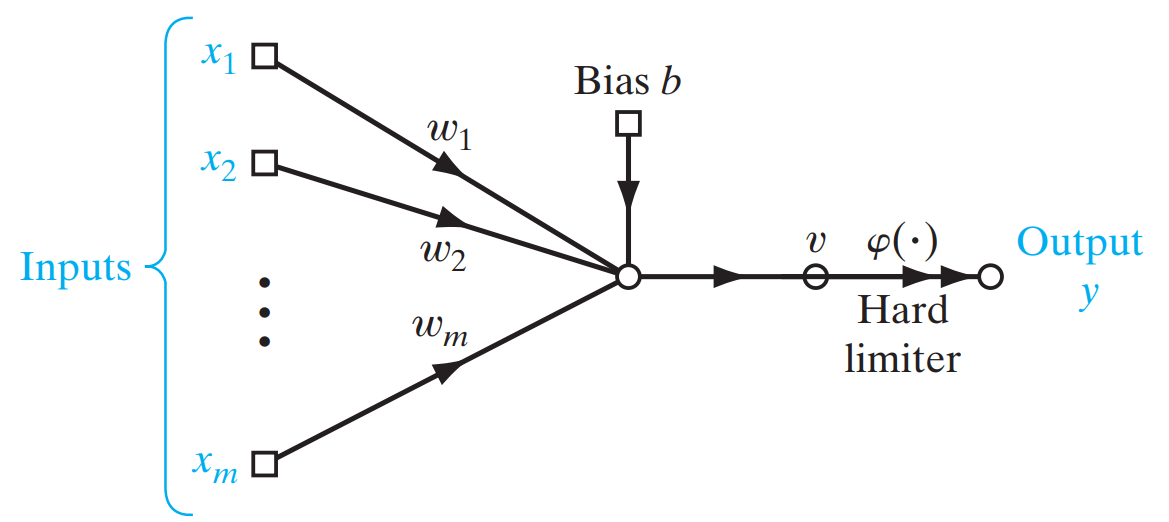
\includegraphics[width=0.65\linewidth]{perceptron.png}
        \caption{A single perceptron}
    \end{figure}

    It has been shown that, if there exist a vector $\boldsymbol{w}*$ such that, for a given set of examples, $y = \xi$ for each example, then the convergence of the perceptron to a solution within a finite number of iterations is assured. Since a perceptron is a linear classifier, it is implied that the existence of a solution goes along with the \textit{separability} of the given set of examples. Such a set is said to be separable if there exist an hyperplane which perfectly splits the positively-classified input vectors and the negatively-classified ones.

    This result, called the \textit{Perceptron Convergence Theorem}, raised great enthusiasm. But few years later, in 1969, Marvin Minsky and Seymour Papert showed that separable problems are more or less whiteflies in a swarm of non-separable problems.

    \subsection{Symmetric circuits and Ising magnets}

    By using a network of perceptrons it is possible to simulate and study an Ising system, i.e. a N-dimensional lattice where each node has only one of two possible states: $S=1$ or $S=-1$. This system is in analogy to a grid of $\frac{1}{2}$-spin atoms. Each atom subject to a magnetic field of intensity $h$ has energy $-hS$.

    We assume that the $i$-th atom interacts with the $j$-th one through the interaction parameter $w_{ij}$. Since in physics systems the interactions are symmetric, $w_{ij} = w_{ji}$. Therefore, the magnetic field perceived by the $i$-th atom is the sum of all the interactions, together with an external magnetic field parameter $\theta_i$:

    $$h_i = \sum_j w_{ij}S_j + \theta_i $$

    This model prescribes that the new state is given by:
    $$S_i' = \text{sgn}\left(\sum_j w_{ij}S_j + \theta_i \right) $$

    These two relations describe respectively the interactions and the dynamics of the model. In the last one, the analogy with the perceptron is obvious. We conclude that an Ising model can be simulated by appropriately connecting a number of perceptrons. A deeper investigation of this model goes behind the goals of this work.


    \begin{figure}[H]
        \centering
        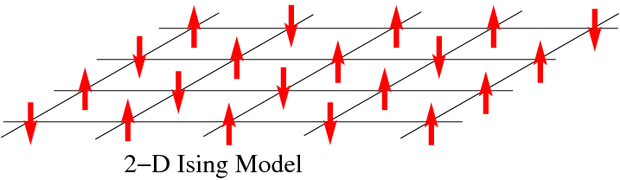
\includegraphics[width=0.65\linewidth]{ising.png}
        \caption{The scheme of a 2-D Ising model}
    \end{figure}














\newpage

\section{Principles of supervised learning}

 In the first part of this chapter we will outline some general concepts of machine learning and model selection, in the perspective of what is called supervised learning. In the second part, we will focus on a very fertile and fast-growing subfield, which is nowadays referred to as Deep Learning.

    \subsection{Learning algorithms}
     Given a set of inputs $\mathbb{X}'$ which is known to have some influence on a set of outputs $\mathbb{Y}'$, the task of using the input to predict the output is called supervised learning. In particular, it is assumed that a function $f(x) = E(Y | X = x) $ exists such that:
     $$ Y = f(X) + \epsilon$$


     The goal in supervised learning is to use a given pair $(\mathbb{X}, \mathbb{Y})$, where $ \mathbb{X}\subset\mathbb{X}'$ and $ \mathbb{Y}\subset\mathbb{Y}'$, to best approximate $f$.

     Algorithms that exploits the input set $\mathbb{X}$ to find a good approximation of $f$, i.e., that are able to learn from data, are called learning algorithms.

         \subsubsection{Loss function}
         Supervised learning algorithms are a subclass of learning algorithms, and they are so called because they benefit from a supervision while guessing the predictions for the elements of the input set. This kind of supervision is implemented by defining a Loss Function $\mathcal{L}$. For each predicted value, $\mathcal{  L}$ will return a real value. The higher the value, the worse is the prediction. In this sense, the Loss is a feedback function for the algorithm, thanks to which it can adjust its parameters to better fit the true outputs for the given inputs.

         We assume a parametric model for the function f, i.e. $f(x) = f(x; w)$, for some parameters vector $w$. On the other hand, $\mathcal{L}(\hat{y}, y_{true})$ is the value returned by the loss function for the prediction $\hat{y}$ with true value $y_{true}$. In response to this value, the parameters $w$ will be modified, according to a specific optimization method, for $\hat{f}(x)$ to better match $y_{true}$, i.e. to reduce the value of $\mathcal{L}(\hat{y}, y_{true})$.
         Therefore, in a machine learning perspective, learning is minimizing a predetermined loss function on a given set of inputs for which the outputs are known.

         The choice of the loss function is key to the problem of building a well performing algorithm. Of course, the more similar are $\hat{y}$ and $y_{true}$ the smaller should be the value returned by $\mathcal{L}(\hat{y}, y_{true})$, but this observation does not narrow it down enough; in fact, the definition of similarity remains undetermined. For this purpose, a suggestion comes from the Principle of Maximum Likelihood, which prescribes to select the parameters $w$ that maximizes the likelihood function $\mathbb{L}$, defined as:

         $$ \mathbb{L} = P(X=x | w)$$

         This principle, applied to the model $ Y = f(X) + \epsilon$, with $\epsilon \sim N(0, \sigma^2)$, returns a loss function called Mean Squared Error, defined as:
         $$ MSE(\hat{y}, y_{true}) = \frac{1}{N} \sum_{n=1}^{N} (\hat{y}_n - y^{true}_n)^{2}$$

         For a classification problem, the maximum likelihood method returns another important loss function, called Cross Entropy:

         $$ H(\hat{y}, y_{true}) = - \sum_{n=1}^{N} \hat{y}_n \log(y^{true}_n)$$

        \subsubsection{Generalization}

        In this paragraph we would like to answer the question: how can we be sure that, if the algorithm learns to perform well on the given dataset $(\mathbb{X}, \mathbb{Y})$, it will behave well also on $(\mathbb{X}'\setminus\mathbb{X},\mathbb{Y}'\setminus\mathbb{Y})$?
        This question addresses what's called the generalization problem, and the answer is that, generally speaking, we can't be sure that our algorithms will generalize. However, in many problems it is reasonable to make the assumption that the outputs are independent and identically distributed (i.i.d.), that is, the true outcome for a particular input is not influenced in any way by the outcomes of the other inputs, and all the outputs follow the same distribution.

        Within this hypothesis, the common practice in supervised learning is to split the dataset into three subsets, called train, validation and test.
        \begin{itemize}
            \item The training set contains the data on which the algorithm, by means of the loss function, will actually optimize its parameters;
            \item The test set contains the data on which, once the training process is concluded, we will measure the performance of our algorithm. The key point is that a performance measure obtained on the same set on which the algorithm has been trained is not trustworthy. In fact, the test set and the training set are disjoint sets.
        \end{itemize}

        The error computed on the test set is sometimes referred to as generalization error. Therefore, saying that a model (i.e. the function implemented by the algorithm at the end of the training process) generalize well means that it obtains a low generalization error, that is, a low error on the test set.

        We will discuss the performance measures and the validation set's role in the following paragraphs.

    \subsection{Model selection}
    In this section, we introduce what's called model complexity, or capacity, and how it affects the performance of a model.

        \subsubsection{Hyperparameters}

        We introduced the parametric function $f(x;w)$ and we mentioned that the optimization consists in changing the parameters' values to reduce the values of the loss function on the training set.
        Unfortunately, for as long as we can change those parameters, we are not assured for the predictions to be satisfactory, not even in the best case. This is due to a simple observation: changing the parameters will not change the complexity of the parametric function. The act of choosing the particular parametric function to be consequently optimized is called model selection.

        To sum up, selecting a model means selecting the family of functions in which, by means of the optimization method, the approximating function will be chosen. The family of function which, in principle, a model can implement is called hypothesis space. Sometime, the features defining the functions' family are called hyperparameters. For instance, given that we want the approximating function to be a polynomial, its maximum degree, which has to be selected a priori, is an hyperparameter of the model.
        That means that to build a model we have to make some guesses on the nature of the statistical process which generated the data, and consequently select a family of approximating functions embedding those hypotheses. The more accurate are these guesses, the more accurate will be the model.

        That said, we could wonder if there exists a class of functions which, on average, is more suitable than some others. That could be a polynomial function with a particular degree, a linear combination of specific exponential and periodic functions, or something more complex. As it may sound reasonable, the answer is that there is no model for which we can say, a priori, that it will be more suitable than another one. This concept is expressed in a famous result, called \textbf{No Free Lunch Theorem} (David Wolpert and William Macready, 1997):

        \begin{displayquote}
            Given a finite set $\mathcal{V}$ and a finite set $\mathcal{S}$ of real numbers, assume that $f:\mathcal{V}\rightarrow\mathcal{S}$ is chosen at random according to uniform distribution on the set $\mathcal{S}^{\mathcal{V}}$ of all possible functions from $\mathcal{V}$ to $\mathcal{S}$. For the problem of optimizing $f$ over the set $\mathcal{V}$, then no algorithm performs better than blind search.
        \end{displayquote}

        In this perspective, it should be clear the reason of defining a validation set: it is a portion of the initial dataset on which different configurations of hyperparameters will be evaluated.


        \subsubsection{Capacity, underfitting and overfitting}

        The No Free Lunch Theorem should not induce to think that all the models are equivalent. In fact, it is not so, and a fundamental property which allows to objectively discriminate between different classes of function is called capacity. Capacity is a loosely defined term, and it can be formulated in several ways. Broadly speaking, it represents the flexibility or the complexity of a space of function. For instance, space of polynomials of degree 12, $\mathcal{P}_{12}$ has a higher capacity of the space of polynomials of degree 8, $\mathcal{P}_8$. That's trivial, but clarifies the main concept: $\mathcal{P}_{12}$ is more flexible than $\mathcal{P}_8$, in fact it contains all the elements of $\mathcal{P}_8$, whereas the opposite it's not true; therefore, we trivially conclude that $\mathcal{P}_{12}$ has a higher capacity than $\mathcal{P}_8$.

        One might be tempted to call into question the validity of the No Free Lunch Theorem, since everything we can achieve by means of a model implementing $\mathcal{P}_8$ is also achievable, a priori, by one implementing $\mathcal{P}_{1 2}$, and therefore the latter should perform better or, in the worst case, the same as the former. What this argument fails to consider is that too much capacity will prevent the model to perform well as well as too little capacity.

        \begin{figure}[H]
            \centering
            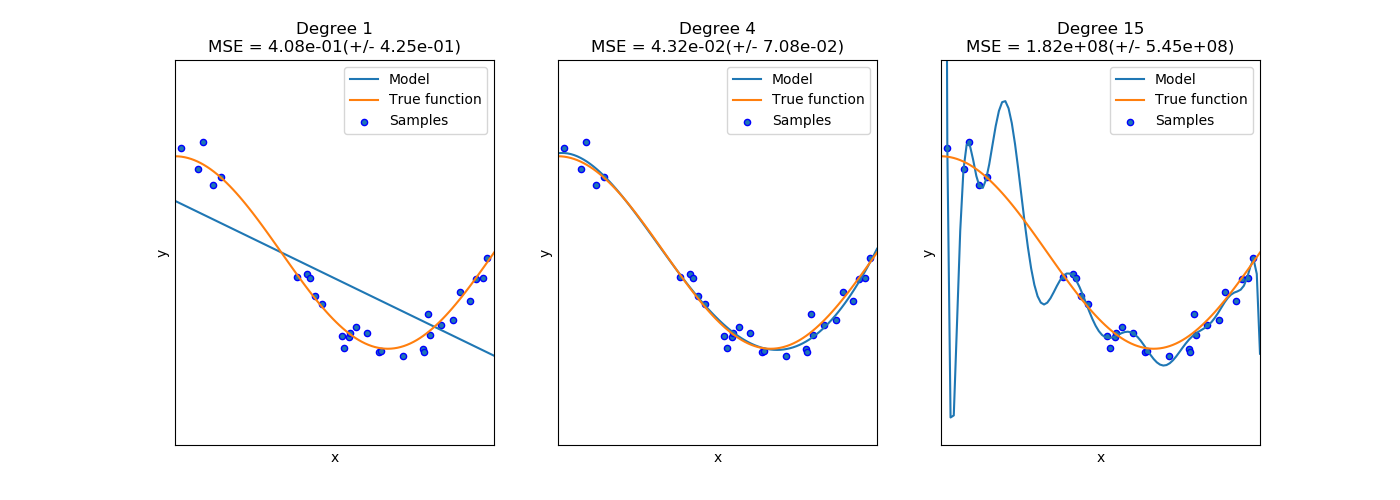
\includegraphics[scale=0.4]{underover.png}
            \caption{Underfitting and overfitting}
            \label{fig:underover}
        \end{figure}

        When the capacity of a model is too low, it will not have the flexibility to well approximate the true function underlying the stochastic process. No matter how big is the dataset or how good is the optimization method, the low capacity impose an inherent boundary to the performance of the model. We will call this complication underfitting.

        A more subtle point concerns the opposite issue, and it arises when the capacity is too high with respect to the complexity of the problem. Since we deal with stochastic processes, the deterministic function producing the observations in our dataset, called data points, is altered by some noise. One risk of having too much capacity is that our model will fit the noise to a certain extent, reducing the training error but undermining the generalization to different sets of points.

        A model with high capacity has one more drawback: many parameters. In fact, Assuming that a model has $N$ parameters, optimizing the model means looking for a good configuration in a $N$-dimensional space. The higher is N, the more difficult is that we find the right solution. This problem is addressed with the name of curse of dimensionality. Interesting geometrical and statistical considerations could be mentioned about it; unfortunately, they go behind the aims of this work.

    \subsection{Regularization}
    Underfitting and overfitting are not symmetrical scenarios. In fact, whereas there is no chance that a low capacity model will find a well performing solution within its hypothesis space, an high capacity model has that chance, even if very subject to the risk of overfitting. A common practice is to take an overfitting model to reduce its hypothesis space, in accordance with a set of preferences aligned with the specific task for which our machine learning algorithm has been designed. This practice is called \textbf{regularization}.

    There exists many ways to regularize a model, and their effectiveness very depends on the given dataset and model. One of the most common and straightforward way to regularize a model is by adding a \textit{penalty} to the loss function, that is, an additive term $\alpha \Omega(\boldsymbol{\theta})$:

    $$\widetilde{\mathcal{L}} = \mathcal{L}(\boldsymbol{\theta}; \boldsymbol{X}, \boldsymbol{y}) + \alpha \Omega(\boldsymbol{\theta})$$

    where $\alpha$ is a non-negative number weighting the contribution of $\Omega(\boldsymbol{\theta})$; $\Omega(\boldsymbol{\theta})$ is a function of all the weights of the model and typically increases with the norm of the weights vector $\boldsymbol{\theta}$. Its effect is to discourage the optimization process from settling the model to some configurations of the parameters for which, a priori, we can reasonably say they won't generalize well.

    Even if, in principle, we are not cutting of any function from the hypothesis space, by applying a penalty term to the loss function we are reducing the probability of the model to implement a number of overfitting function, and it can be considered a kind of capacity reduction. Of course, the intensity of the regularization is weighted by the coefficient $\alpha$, which is an hyperparameter of the model.

   Next up, we shall introduce the two most common norm penalties.

   \subsubsection{$L^2$ regularization}

   The $L^2$ parameter norm penalty is commonly known as $\textbf{weight decay}$, since it discourage the weights to get high values. It is obtained by the previous formula by setting

   $$\Omega(\boldsymbol{\theta}) = \frac{1}{2} \left\|\boldsymbol{w}\right\|_2^2$$

   so that the loss function is

   $$\widetilde{\mathcal{L}} = \mathcal{L}(\boldsymbol{\theta}; \boldsymbol{X}, \boldsymbol{y}) + \frac{\alpha}{2} \boldsymbol{w}^T \boldsymbol{w} $$

   By studying the effect of the norm penalty on the gradient of the loss function, we can gain some insight on how the vector $\boldsymbol{w}* = arg min_{\boldsymbol{w}} L(\boldsymbol{w})$ is transformed by the weight decay. By performing simple manipulation of the gradient and by applying a quadratic approximation of the loss function in the neighborhood of the value of the weights that minimizes the unregularized loss, $\boldsymbol{w}$, we get to the conclusion that the $L^2$ regularization's effect is to rescale $\boldsymbol{w}$ along the axes defined by the eigenvectors of the hessian matrix of the loss function $\mathcal{L}(\boldsymbol{\theta})$ with respect to $\boldsymbol{w}$. As a consequence, all directions along which the parameters does not contribute significantly are decayed away throughout the training process.

   \subsubsection{$L^1$ regularization}
   Another way to reduce the model's complexity is by applying the so-called $L^1$ regularization on the model parameters $\boldsymbol{w}$, which is defined as:

   $$\Omega(\boldsymbol{\theta}) = \left\|\boldsymbol{w}\right\|_1 = \sum\limits_{i} |w_i| $$

   As a consequence, the loss function has the form:

   $$\widetilde{\mathcal{L}} = \mathcal{L}(\boldsymbol{\theta}; \boldsymbol{X}, \boldsymbol{y}) + \alpha \left\|\boldsymbol{w}\right\|_1 $$

   The $L^1$ regularization results in a \textbf{sparse} solution, that is, a solution where some parameters are appropriately set to zero. The sparsity property is a feature selection mechanism, in so far as it simplifies the problem by selecting what features should be used and what should be neglected.

   Different forms of regularization will be introduced in the next paragraphs, within a deep learning perspective.


    \subsection{Performance Measures for classification problems}

    In this paragraph we start to establish the framework of the underlying work of this thesis, which is described in detail in Chapter 4, and we introduce some observations related to the evaluation of a model.

    Since it does not exists a natural measure for evaluating the performance of a model, the metrics we choose strongly depends on the given problem and it reflects our preferences and trade-offs concerning the solution we want to obtain.

    The problem upon which is developed this work is defined as a binary classification problem, since the task is to classify every input as one between two classes. An input is a sequence corresponding to the signal collected for a breath of a patient subject to mechanical ventilation; every breath can contain or not an asynchrony: these two options define the two classes.

    \subsubsection{Confusion matrix}

    Given a dataset associated to a classification problem and a set of predictions obtained by the model we want to evaluate, the confusion matrix is a matrix where each row represents the instances in a predicted class while each column represents the instances in a true class; as a consequence, for a multi-classification problem with $N$ class the confusion matrix is a $N \times N$ matrix.

    In the particular case in which $N = 2$, we can label the two classes as \textit{positives} and \textit{negatives}. Moreover, the confusion matrix takes the simple form of a $2 \times 2$ matrix and it highlights four quantities of great importance:


    \begin{wrapfigure}{r}{0.5\textwidth}
  \begin{center}

     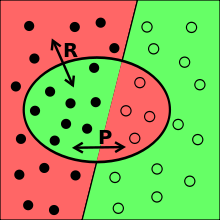
\includegraphics[width=0.6\linewidth]{220px-Recall-precision.png}
     \caption{The black dots represent the positive elements; the empty are dots the negative ones. The green area contains the dots which were correctly classified (TP and TN), while the red area those who were associated with the wrong class (FP and FN).}
  \end{center}
\end{wrapfigure}


    \begin{figure}[H]
    \centering
    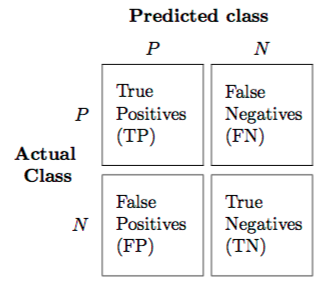
\includegraphics[width=0.5\linewidth]{confusion_matrix_1.png}
    \caption{Binary confusion matrix}
    \end{figure}

    Accuracy, i. e. the ratio of correctly classified examples, is defined as:
    $$Accuracy = \frac{TP + TN}{TP + FN + FP + TN} $$
    Although accuracy is a common performance measure, it is not appropriate for our specific problem, since our dataset is unbalanced, i.e. the number of elements belonging to one class is significantly bigger than the number of elements which belong to the other one.


    Precision is a measure of the model's accuracy over all the examples predicted as positive, and it is defined as:
    $$ Precision = \frac{TP}{TP + FP}$$

    We look for an high precision when the circumstances require a low number of false alarm. On the other hand, if the priority is to limit as much as possible the number of missed positives, the performance measure we should pay attention to is the recall, or sensitivity, defined as:

    $$ Recall = \frac{TP}{TP + FN} $$

    Notice that focusing on maximizing one of these two last measures with no regard for the other one can result in a very poor overall performance. For instance, if we put all our attention and efforts on having the highest recall, that is equivalent to minimizing the false negatives, we could obtain a model which, to do so, will naively predict almost all of the examples as positive. In this circumstance, we will get a very high recall, even 1.0, but, on the other hand, the number of false positives will be also very high, resulting in a low precision.

    It is clear that precision and recall should always be considered together, if necessary with different weights. Within this perspective, we define a more general measure which has precision and recall as special cases. It is called $F_{\beta}$ score, and it is defined as:

    \begin{equation*} \label{eq1}
    \begin{split}
    F_{\beta} & = (1 + \beta^2)\frac{precision \cdot recall}{(\beta^2 \cdot precision) + recall} \\
     & = \frac{(1 + \beta^2) \cdot TP}{(1 + \beta^2) \cdot TP + \beta^2 \cdot FN + FP}
    \end{split}
    \end{equation*}

    where $\beta$ is a non-negative real number. For $\beta = 0$, $F_{\beta}$ produces the precision; on the other hand, as $\beta$ gets higher values $F_{\beta}$ will be closer and closer to the recall measure. In this work, we set up $\beta = 2$, since we consider a priority to reduce the false negatives while keeping the false positives' number under control.



















\newpage
\section{Deep Representations}
%intro sul deep learning
In this chapter we introduce some key concepts of Deep Learning, a term referring to the subfield of Machine Learning which studies brain-inspired algorithms, called Artificial Neural Networks. Although the idea of algorithms inspired by the synaptic processes taking place in a biological brain was for the first time implemented, as far as we know, in 1943, when Warren McCulloch and Walter Pitts proposed the first artificial neuron algorithm, the term \textit{Deep Learning} is relatively new, and has spread incredibly fast in recent years. This term somehow fits the structure of the modern neural networks, highlighting the particular feature which, arguably, deserves the credits for their effectiveness towards a broad family of problems: the depth. As we will discuss in the following paragraphs, this models are built by combining many nonlinear transformations, so that complex features underlying the given data points can be learned.

    \subsection{Output units}
    To get a convenient and flexible visualization, we formalize a model as a directed graph where each node represents a vector or a scalar. When two or more nodes point to a new node, its vector is the result of an operation between them. The operation is usually specified near the new node if not implied by the context.

    This structure is called \textbf{computational graph} and, ultimately, it unambiguously represents a function, which is in our case the approximating function for a statistical model.

        \subsubsection{Logistic layer}

        For instance, let's take the logistic regression model, which is defined by the following predictive function:

        $$ \hat{y} = \sigma(\boldsymbol{x}^T\boldsymbol{w} + b) $$

        where


        $$\sigma(z)  = \frac{1}{1 + e^{-x}}$$

        The computational graph associated with this predictive model is sketched as follows:

        \begin{figure}[H]
        \centering
        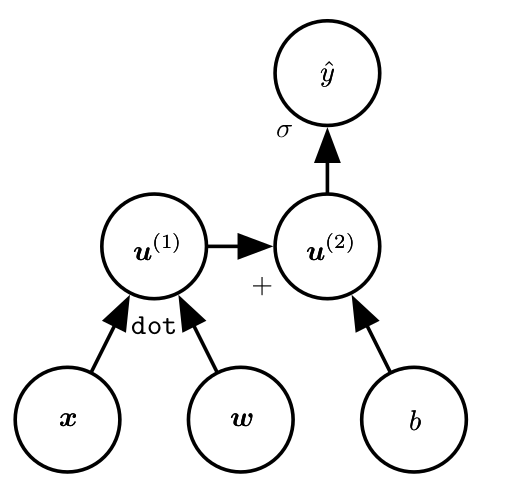
\includegraphics[width=0.4\linewidth]{compgraph.png}
        \caption{Computational graph associated with a logistic regression}
        \end{figure}

        Notice that the lower five nodes, together with their operations, simply correspond to an affine transformation of the input vector $\boldsymbol{x}$. Eventually, the last operation, indicated with $\sigma$, applies a nonlinear transformation, called \textbf{activation function}. As we shall soon see, in deep learning's computational graphs a set of nodes and operations which apply a nonlinear function to the result of an affine transformation is a common structure, and it is usually called \textbf{layer}. In fact, an artificial neural network is, generally speaking, an algorithm which, layer by layer, alternates affine and nonlinear transformations to a given input, ultimately producing an output.

        A layer is characterized by its activation function. The computational graph we just introduced implements what is called a \textbf{logistic layer}. Since the logistic function's output is a number belonging to the interval $]0, 1[$, for binary classification problems it is the standard to end the artificial neural network with a logistic layer. In this way, for a given input the model returns a number expressing a degree of confidence, that is, the probability for that input to be a positive instance of the underlying problem.

        \subsubsection{Softmax layer}

        For a multiclass classification problem, we expect a model to return a probability distribution over all the possible classes. For the binary case, instead, we were demanding for the output to be a single number:
        $$ \hat{y} = P(y = 1 | \boldsymbol{x}) $$
        To generalize to an N-classes classification problem, we need our model to produce a vector $\boldsymbol{\hat{y}} \in [0,1]^N $, with $\hat{y}_i = P(y = i | \boldsymbol{x}$. Also, since we want $\boldsymbol{\hat{y}}$ to represent a distribution over N classes, we require the normalization condition to be true, that is:
        $$ \sum\limits_{i} \hat{y}_i = 1 $$
        This properties are provided by the softmax function, defined as:
        $$softmax(\boldsymbol{z})_i = \frac{\exp{z_i}}{\sum\limits_{j} \exp{z_j}} $$

    \subsection{Hidden units}

        So far we have we've focused on the last layer of a computational graph, which is called output layer. In the most part of parametric machine learning models an output layer can be identified, just as in linear or logistic regressions.

        We now introduce the very peculiarity of neural networks models: the hidden layers. An hidden layer consists in an additional transformation applied to the input data, and it is so named because it is located before the output layer. The effect on the approximating function implemented by the model is to add a new composition, so that:
        $$\hat{\boldsymbol{y}} = f(\boldsymbol{x}; \boldsymbol{w}_f) \rightarrow \hat{\boldsymbol{y}} = (f \circ h)(\boldsymbol{x}; \boldsymbol{w}_h, \boldsymbol{w}_f) $$

        where we assume compatibility between $h$'s range and $f$'s domain.

        The number of hidden layers is the very factor which naturally led to an evolution of this field in recent years, also justifying the name change we mentioned before. In fact, in Deep Learning \textit{deep} refers to the architecture of the model, which consists in the overlapping of a considerable number of layers. The output layers is, of course, only the last one, which produces the final output. Everything else between the input layer and the output layer is a hidden layer. The number of hidden layers can range from one, for a simple model with enough complexity to solve the XOR problem, to 152 for ResNet-152. A modern technique, called \textit{stochastic depth} allow to have even more then one thousand layers with an increase in performance over common datasets used in research, like CIFAR-10, CIFAR-100, SVHN.

        \begin{figure}[H]
        \centering
        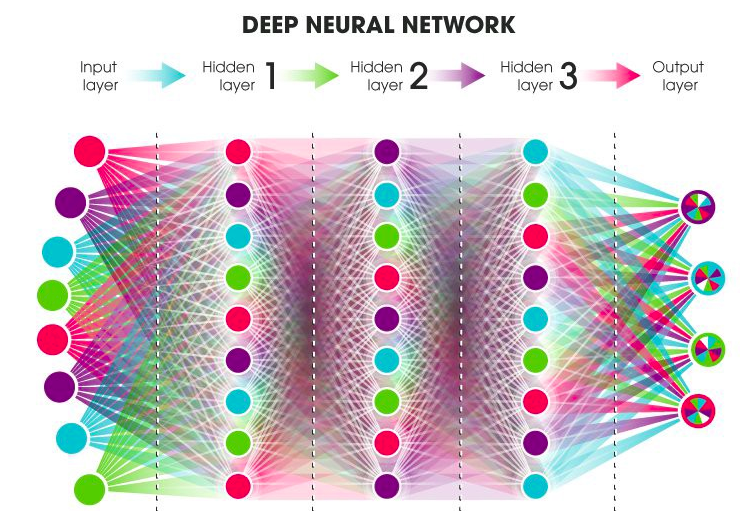
\includegraphics[width=0.6\linewidth]{dnn.png}
        \caption{Visualization of a 5-layers neural network}
        \end{figure}

        \subsubsection{ReLU layer}
        The most common activation function used for hidden layers in recent years is called Rectified Linear Unit, ReLU, defined as:

        $$g(\boldsymbol{z}) = \max(0, \boldsymbol{z}) $$

        The complete transformation applied by a layer on its input \textbf{x} is, therefore:

        $$\boldsymbol{x} \rightarrow \boldsymbol{z} = \boldsymbol{W}^T \boldsymbol{x} + \boldsymbol{b} $$
        $$\boldsymbol{z} \rightarrow g(\boldsymbol{z}) =\max(0, \boldsymbol{z}) $$


        \begin{wrapfigure}{1}{0.4\textwidth}
            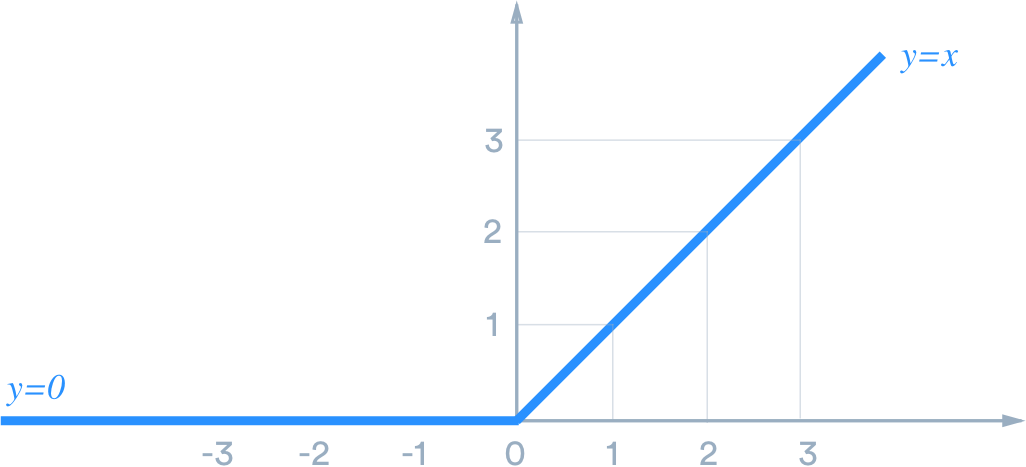
\includegraphics[width=1\linewidth]{relu.png}
            \caption{ReLU's plot}
            \label{fig:relu}
        \end{wrapfigure}

        As we will see in the next paragraph, a fundamental feature of an activation function is differentiability. Since activations are always element-wise, their domain is $\mathbb{R}$, therefore differentiability simply requires the existence of the first derivative. In contrast with that, should be noticed that the ReLU activation is not differentiable in zero. Luckily, this is not an issue, for two relevant reasons whose validity can be extended to any other function which is differentiable \textit{almost everywhere}:

        \begin{itemize}
            \item the probability of getting a zero-input is quite small;
            \item in a real numbers' finite representation, like the one applied by a machine, there is an error given by each computation which does not allow us to be sure that a zero really was a zero.
        \end{itemize}

        Therefore, non-differentiability in few, isolated points is not an issue. Moreover, non-differentiable activations can be always generalized to differentiable functions without any sensible loss in performances.


    \subsection{Gradient Descent}
    Arguably, the two central problems  in machine learning concerns respectively hyperparameters and parameters:
    \begin{itemize}
        \item \textbf{Hyperparameters}: Finding a good model architecture, i.e. a family of approximating function, to solve the given problem;
        \item \textbf{Parameters}: Finding optimal parameters' values for the selected architecture and the given problem.
    \end{itemize}

    So far, we focused on the first aspect. Now, we want to consider the second problem, introducing a simple rule to incrementally update the parameters towards a configuration which, hopefully, will produce a good performance on our problem:

    $$\boldsymbol{\theta} \leftarrow \boldsymbol{\theta} - \epsilon  \textbf{g} $$

    where $\boldsymbol{\theta}$ represents all the model's parameters, $\boldsymbol{g}$ is the gradient of the loss function with respect to $\boldsymbol{\theta}$, and $\epsilon$ is a positive, typically small number called \textbf{learning rate}.

    The idea behind is simple: since we want to minimize the loss function, we move our parameters vector $\theta$ by a little step towards a position where the loss function is lower. This procedure is repeated until a local minimum is reached.

    \begin{figure}[H]
        \centering
        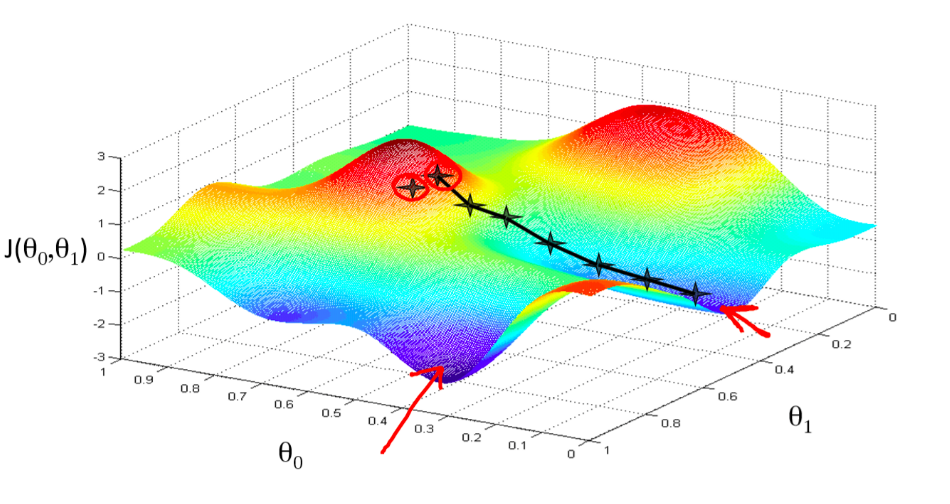
\includegraphics[width=0.75\linewidth]{gradientdescent.png}
        \caption{Visualization of the gradient descent on weights $\theta_0$ and $\theta_1$ by means of the loss function J}
    \end{figure}

    In the picture above, the arrow on the right indicates the weights configuration reached by means of the gradient descent rule, and it is a local minimum. However, it is not the global minimum of the given loss function, which is pointed by the left arrow.

        \subsubsection{Momentum correction}

        There are many optimization methods which, starting from the gradient descent, apply corrections to the rule: RMSprop, Adaptive Moment Estimation (ADAM), Nesterov Accelerated Gradient (NAG), and many more.

        All these methods insert in the weights' update a factor called \textit{momentum}, or \textit{inertia}, which prevents the parameters vector to make sharp variations on its path towards a minimum. A definition which holds for all the mentioned methods is that the total velocity at iteration t+1 is given by:

        $$v_{t+1} = \theta_{t+1} - \theta_t$$

        However, different methods have different velocity definitions. The classical momentum correction has been defined as:

        $$ v_t = \mu_{t-1} v_{t-1} - \epsilon \nabla \mathcal{L}(\theta_{t-1}) $$

        So that the full update rule is:

        $$ \theta_{t+1} = \theta_t + \mu_t v_t - \epsilon_t \nabla \mathcal{L}(\theta_t)$$

        The Nesterov Accelerated Gradient method prescribes to look ahead in the evaluation of the gradient:

        $$ \theta_{t+1} = \theta_t + \mu_t v_t - \epsilon_t \nabla \mathcal{L}(\theta_t + \mu_t v_t) $$

        \begin{figure}[H]
            \centering
            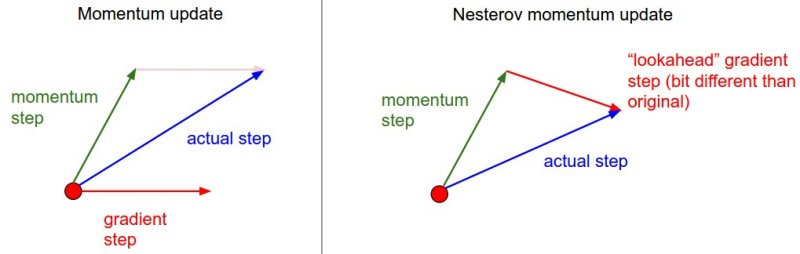
\includegraphics[width=0.9\linewidth]{nesterov.jpeg}
            \caption{Classical momentum correction compared to Nesterov's one}
        \end{figure}

        As a result of the momentum term, the we gain faster convergence and reduced oscillation.
        More complex methods, like ADAM or RMSprop, explore the local geometric properties of the parameters space and, in addition to correcting the step's direction, they fine-tune the learning rate parameters.


        \subsubsection{Backpropagation algorithm}

        So far we have discussed about methods which use the loss gradient computed in some points of the parameters space to update the network's weights. Now we want to briefly address the problem which arises when computing the gradient for the loss function of a deep learning model.

        Firstly, we remind the so-called \textbf{chain rule of calculus}. Let $g$ be a function mapping $\mathbb{R}^m$ to $\mathbb{R}^n$, and $f$ a map from $\mathbb{R}^n$ to $\mathbb{R}$. Also, suppose that $\boldsymbol{y} = g(\boldsymbol{x})$ and $z = f(\boldsymbol{y})$. Then:

        $$ \frac{\partial z}{\partial x_i} = \sum_{j=1}^n \frac{\partial z}{\partial y_j} \frac{\partial y_j}{\partial x_i}$$

        In vector notation:

        $$ \nabla_{\boldsymbol{x}} z =\left( \frac{\partial \boldsymbol{y}}{\partial \boldsymbol{x}} \right)^T \nabla_{\boldsymbol{y}} z $$

        where $\left( \frac{\partial \boldsymbol{y}}{\partial \boldsymbol{x}} \right)^T$ is the $n \times m$ Jacobian matrix of $g$ with respect to $\boldsymbol{x}$.

        When applying the chain rule to a computational graph, if we just compute the gradient for each node lying over any path from the input node to the loss node, we are subject to an exponential explosion of repeated computations with respect to the number of edges in the graph, since we have to compute the same Jacobian matrices more and more time.

        The backpropagation algorithm addresses this issue, and it requires an amount of computations which scales linearly with the number of edges. To be exact there are many backpropagation algorithms, with different levels of complexity and optimization, but the core idea is simple: performing a backward computation from the output layer to the input layer, each time evaluating the partial derivatives and memorizing their value to reuse it in the next step.

    \subsection{Convolutional neural networks}
        In this paragraph we briefly describe a specific kind of architecture, known as convolutional neural network, which is in its simplest form a feed-forward structure with a number of convolutional layers followed by a densely connected output unit. \textit{Densely connected} simply refers to the fact that the unit's weights are, in general, different from zero, although they can be very small.

        \subsubsection{Convolutional layer}

        The convolution operation is defined as:

        $$ p(t) = (x \ast w)(t) = \int \! x(a)w(t-a) \, \mathrm{d}a $$

        In the deep learning terminology, the function $x$ is called \textit{input}, while the second argument, $w$, is the \textit{kernel}. Lastly, the output function $p$ is said \textit{feature map}.

        Since we work with digital data, every signal is represented by a time series, i. e. the time variable $t$ is discretized. The convolution operation is, therefore, the limit of a sum:

        $$p(t) = (x \ast w)(t) = \sum_{a = -\infty}^{+\infty} x(a) w(t-a) $$

        Convolutional neural networks (CNN) success is mainly due to three nice properties of the convolution operation:

        \textbf{Sparse interactions}: traditionally, each output interacts with each input, since a matrix multiplication is performed. In CNN, kernels are definitely smaller than the input, since it is made the assumption that the relevant interactions are local. This allows to store fewer parameters, reducing the memory requirements of the model and the number of operations for the output to be computed.

        \begin{figure}[H]
            \centering
            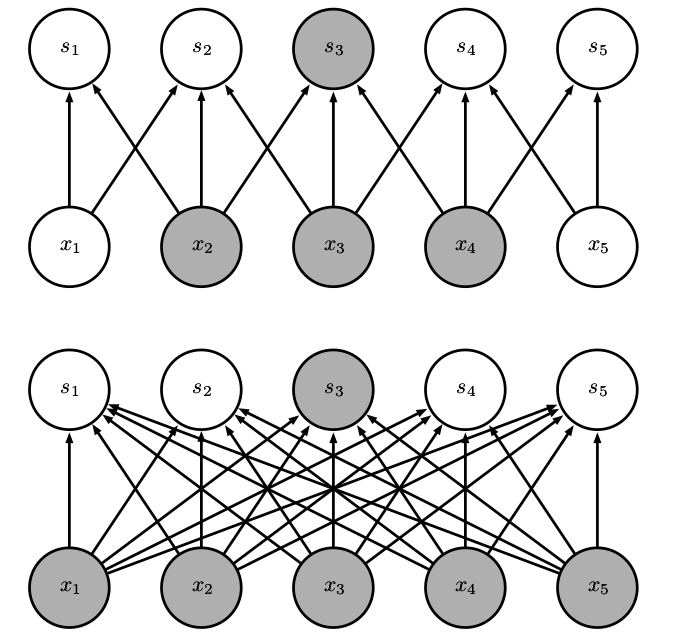
\includegraphics[width=0.6\linewidth]{sparse_connectivity.png}
            \caption{A visualization of sparse connectivity}
        \end{figure}



        \textbf{Parameter sharing}: for a densely connected layer, each weight defines a single interaction between an element of the input and an element of the output, and it is used exactly once during the computation of the output layer. CNNs, on the other hand, have \textit{tied weights}, that means that a relatively small set of weights is shared by a larger set of inputs to produce the next layer's elements.

        \textbf{Equivariant representations}: a function $f$ is equivariant to a function $g$ if $f(g(x)) = g(f(x))$. Let $g$ be a function that shifts the input; therefore, the convolution operation is equivariant to any input's shift. In other words, let's suppose that a specific representation is associated by the convolution to a particular event in the time series. If we shift the same event $N$ time steps later, the output for the shifted sequence will show the exact same representation $N$ steps later (assuming there is no a resizing process within the transformation).


        \subsubsection{Pooling}

        Typically, a convolutional layer's transformation can be split in three steps:
        \begin{enumerate}
            \item A number of $N$ parallel convolutions are performed on the input sequence, producing $N$ linear activations;
            \item To each linear activation, an element-wise nonlinear function is applied;
            \item A \textit{pooling function} is applied to each sequence.
        \end{enumerate}

        A pooling function is a transformation that summarizes the local properties for a certain location within the input sequence. The most common form of pooling is called \textbf{max pooling}, which reports the maximum value within an $L$-timesteps window. This introduces invariance to small translations of the sequence, shrinking the information and reducing the number of parameters needed for the following layers.


    \subsection{Regularization in deep learning models}

        We already introduced regularization, showing how a model's loss function can by modified to reduce the chance of overfitting. We now briefly introduce two regularization techniques which are very common and were specifically developed within the deep learning scenario. In fact, for deep neural nets overfitting is a serious problem, which requires solutions carefully built through observations made upon their particular architecture.

        \subsubsection{Dropout}
        Dropout is a simple yet powerful stochastic regularization technique that reduces overfitting with negligible computational cost. It was introduced by Srivastava et al. in 2014. Since than, it has been nearly a must-have for every deep architecture.
        For dropping out a neuron we mean removing it from the network for that specific iteration. In particular, it is implemented by assigning to each neuron of a layer a probability $p$ for its output to be multiplied by zero just for that specific training iteration. The probability $p$ is usually set to a number between $0.25$ and $0.5$ during the training process, and always to $0.0$ during the validation and the test iterations.

        \begin{figure}[H]
            \centering
            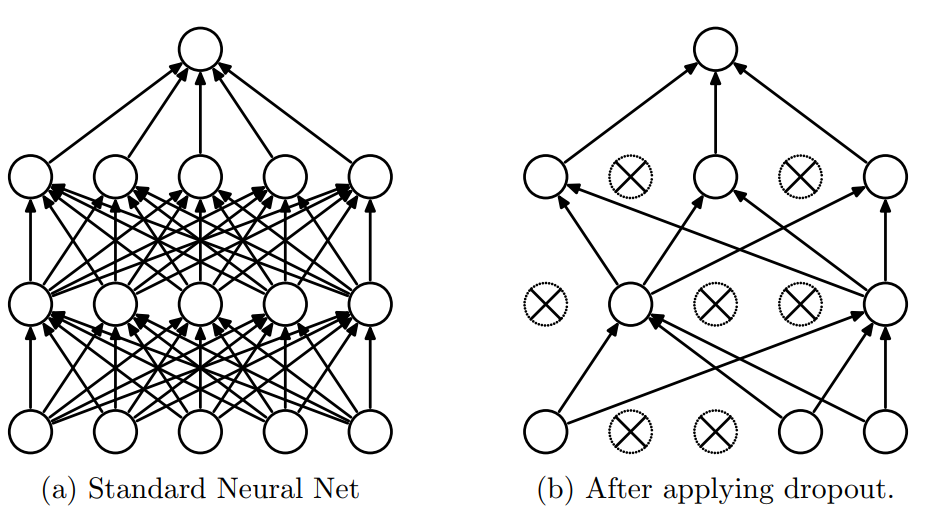
\includegraphics[width=0.6\linewidth]{dropout.png}
            \caption{How dropout works}
        \end{figure}


        Dropout can be interpreted as a form of model averaging and, at the same time, a noise-injection method. Although the reason of its effectiveness relies upon sensitive considerations on the \textit{bagging technique}, which is not discussed in this work, it is intuitive that randomly dropping out some neurons at each forward step prevents some units to co-adapt along features which are not representative of the stochastic process generating the data.


        \subsubsection{Batch Normalization}

        As we previously highlighted, depth is what allows a neural network to capture the most subtle underlying features of a stochastic process. Despite it, depth is also the cause of many issues which arise during the training process, eventually leading to poor performance on the test set or to a slow convergence.

        An important factor which slows down convergence is called \textit{internal covariate shift}. It refers to the fact that, during the training, the parameters of each layers change at each iteration. As a consequence, since the input to the $i$-th layer depends in the $(i-1)$-th layer's parameters, the input distribution for the $i$-th layer changes at each iteration. The magnitude of its change depends on the learning rate: if it is very small, the internal covariate shift is negligible but for the convergence many training iterations will be required; on the other hand, if learning rate is high, the changed input distribution will shift some components of the input vector towards the saturated regime of the nonlinearity, and it also will slow down the convergence. Also, as the network's depth increases, layer after layer we get a snowballing effect.

        The \textbf{batch normalization} addresses this issue by applying the \textit{Batch Normalizing Transform} to the input $x$ over a minibatch $\mathcal{B} = \{ x_1, \dots , x_m \}$.

        \begin{figure}[H]
            \centering
            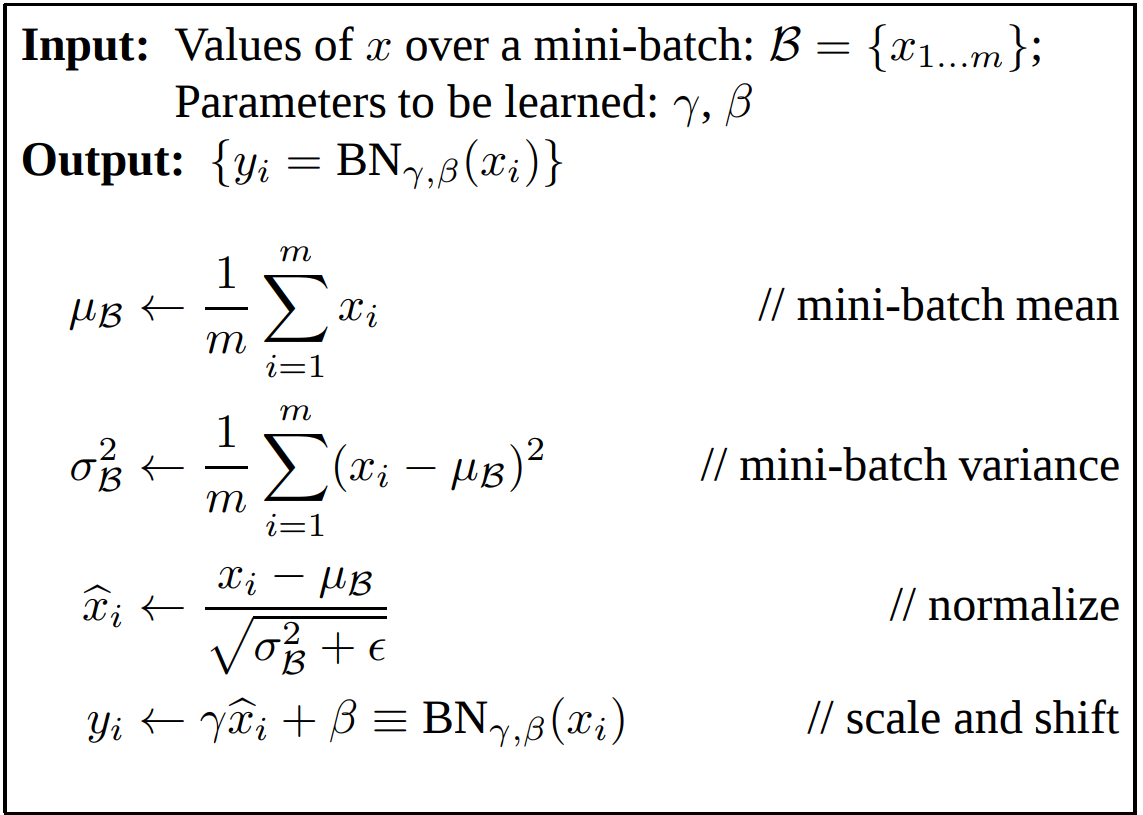
\includegraphics[width=0.75\linewidth]{batch_normalization.png}
            \caption{Batch Normalizing Transform algorithm}
        \end{figure}

        In the algorithm above, $\epsilon$ is a constant added to the minibatch for numerical stability; $\beta$ and $\gamma$ are respectively the shifting and scaling parameters, which are to be learned. In so doing, each layer's input distribution is scaled and shifted in such a way to increase the performance. Notice that $\beta$ and $\gamma$ are not hyperparameters: they are to be learned through gradient descent, just as any other weight.















\newpage

\section{Mechanical Ventilation and Asynchronies}

    \subsection{Respiratory mechanics}

    Pulmonary ventilation is one of the primary mechanism of the respiration process, consisting in the alternation of inhalation and exhalation. Inhalation corresponds to an increase in lung volume, which is the result of an active contraction of the diaphragm. On the other hand, exhalation exploits the lungs' elasticity to expel the inhaled air, and it brings to a decrease in lung volume. In rest conditions, therefore, the exhalation is a passive process and only during the inhalation there is an active effort of the patient. However, the former can be actively speeded up by using the abdominal muscles.

    The work produced by the patient during the pulmonary ventilation, called work of breathing (WOB), at rest coincides with the inhalation work generated by the forces the patient's muscles apply in order to decrease the lung volume. For physiological systems, like the one we are considering, it is easier to measure pressures than forces. Therefore, we will quantify the mentioned quantities, together with the way in which they influence each other, by means of the pressure.

    \subsubsection{Equation of motion for the respiratory systems}



    \begin{wrapfigure}{1}{0.4\textwidth}
        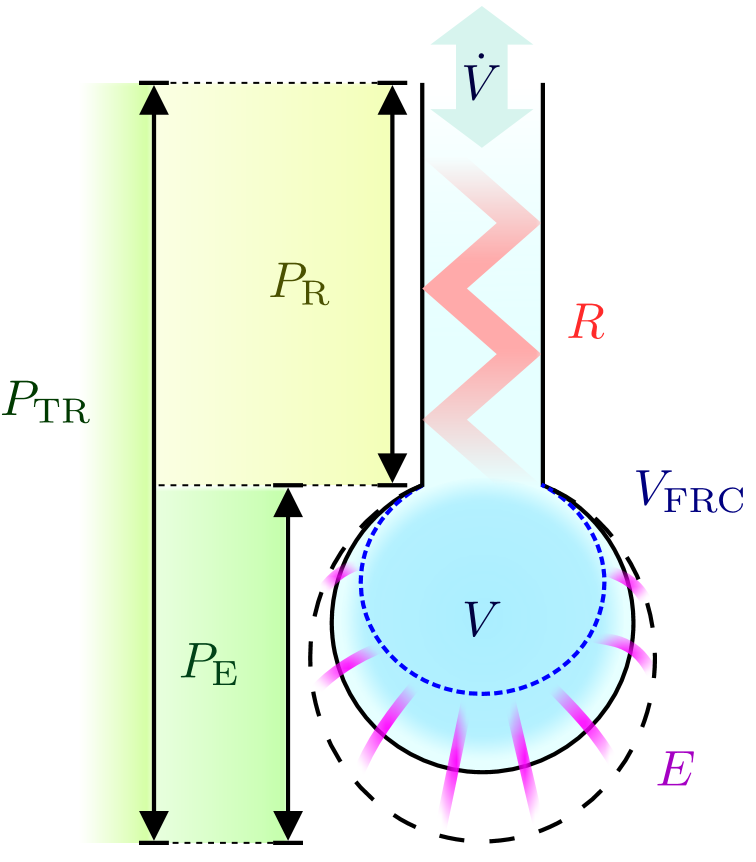
\includegraphics[width=1\linewidth]{PulmVenti.PNG}
        \caption{Diagram of the described model}
        \label{fig:pulmvent}
    \end{wrapfigure}

    Let's think of the respiratory system as an elastic chamber, corresponding to the lungs, and a tube connected to the atmosphere, corresponding to the airway. Together with this scheme, we consider the following time-dependent variables, which describe the state of the system:
    \begin{itemize}
        \item $V$: the volume of the chamber, i.e. the volume of the air contained in it;
        \item $\dot{V}$: the flow of the air through airway, that is, the derivative of volume with respect to time;
        \item $P$: the pressure on the surface of the chamber.
    \end{itemize}
     The relation among them is described by the equation of motion for the respiratory system, which is derived from the force-balance equation:
     $$ P_{TR} = P_E + P_R $$
     where $P_{TR}$ is the trans-respiratory pressure, i.e. the difference between the pressure at the airway opening and the atmospheric pressure, $P_E$ is the pressure due to the elasticity of the chamber, which induce an elastic recoil on the surface, and $P_R$ is the pressure due to the resistance to the transition of the air through the airway.

     These quantities can be expressed in terms of the variables we defined above. Let $V_{RFC}$ be the volume of the chamber at rest, called the residual functional capacity. By defining $\Delta V = V - V_{RFC}$, we can express $P_E$ as a product $\Delta V$ and a fixed quantity $E$, called elastance. On the other hand, $P_R$ is proportional to the flow, and we call the multiplicative constant $R$ resistance:
     $$ P_E = E\Delta V \quad \textrm{and} \quad P_R = R\dot{V} $$

     In absence of external devices, the trans-respiratory pressure corresponds to the pressure produced by the respiratory muscles, $P_{mus}$, so that the equation of motion becomes:
     $$ P_{mus} = E\Delta V + R\dot{V} $$
     From this relation, we derive the expression of the flow,
     $$ \dot{V} = \frac{P_{mus}-E\Delta V}{R}$$
     whereby it is clear that, in absence of muscular efforts, i.e. $P_{mus}=0$, the system's volume naturally converges to $V_{RFC}$.

    \subsection{Mechanical Ventilation}
    The previous equation are derived for a system which is free of any external device, in fact only the muscular pressure contributes to left member of the equation of motion.

    \begin{wrapfigure}{1}{0.4\textwidth}
        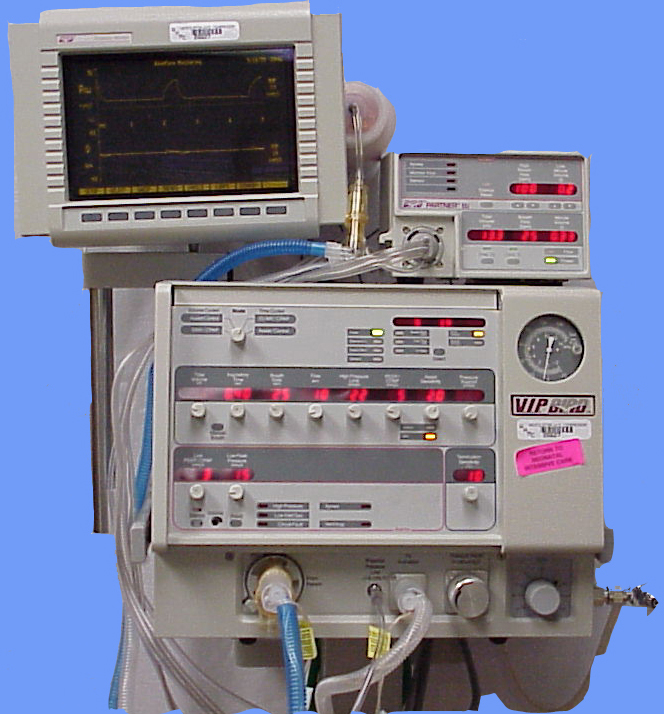
\includegraphics[width=1\linewidth]{mechanicalventilator.jpg}
        \caption{A mechanical ventilator}
        \label{fig:mecvent}
    \end{wrapfigure}

    It should be clear at this point that all the work produced by the patient, what we called the WOB, is due to the muscular pressure he has to exert. As mentioned at the beginning of this chapter, the aim of a mechanical ventilator is to reduce the patient's effort, performing a part or the whole of the WOB. So, in presence of a mechanical ventilator, the equation of motion has to be modified into the equation of motion for mechanically assisted pulmonary ventilation:
    $$ P_{mus} + P_{vent} = E\Delta V + R\dot{V} $$

    This equation describes the patient-ventilator interaction, and it shows how, by controlling one variable, we undirectly control the other two. In fact, a first constraint is given by the relation between volume and flow:

    $$ \frac{dV}{dt} = \dot{V} $$
    The second one is, of course, the equation itself.
    This considerations brings us to the idea that a mechanical ventilator needs to work towards a single variable, pressure or volume, to assist the patient. This is key to the definition of a taxonomy for the different modes in which mechanical ventilators works, that is, how do they interact with the patient.

    \subsection{Ventilation modes}
    All the aspects of the patient-ventilator interaction together define what is called ventilation mode. An in depth discussion of the different ventilation modes is not among the aims of this thesis. In fact, even though the data used in the following analysis have been collected under different known modes, this kind of information does not constitute a relevant feature in our approach.

    \subsubsection{Breathing patterns}
    The breathing pattern is defined by the combination of two choices:
    \begin{itemize}
        \item \textbf{Control Variable}: it defines which one of the three variables (pressure, volume, flow) will be regulated by the MV; the common choice is between pressure-controlled (PC) and volume-controlled (VC) mechanical ventilators;
        \item \textbf{Breath Sequence}: it determines how rigid is the breathing schedule imposed by MV.
    \end{itemize}

    We define a spontaneous breath as a breath for which the patient defines both the start (trigger) and the end (cycling) of every inhalation. If the trigger and/or the cycling is handled by the MV, the breath is said to be mandatory.

    The most common breath sequences are:

    \begin{itemize}
        \item \textbf{Continuous Mandatory Ventilation (CMV)}: the ventilator delivers a mandatory breath every time the patient makes an inspiratory effort;
        \item \textbf{Intermittent Mandatory Ventilation (IMV)}: between mandatory breaths, spontaneous breaths are permitted;
        \item \textbf{Synchronized Intermittent Mandatory Ventilation (SIMV)}: similar to the IMV, but the mandatory breath is triggered by the patient;
        \item \textbf{Continuous Spontaneous Ventilation (CSV)}: all breaths are spontaneous.
    \end{itemize}

    \subsubsection{Neurally Adjusted Ventilatory Assistance}
    To the PC-CSV pattern can be applied an extra feature, called Neurally Adjusted Ventilatory Assistance (NAVA). By means of NAVA, the mechanical ventilator is able to exploit the EAdi signal (electrical activity of the diaphragm signal), which is picked up by an esophageal probe and represents an accurate measure of the patient voluntary inspiratory efforts.

    \subsection{Asynchronies}
    A crucial point in the mechanical ventilation is that the device and the patient are well synchronized or, better, that the MV smoothly supports the patient's voluntary breathing attempts. In fact, for the MV to effectively reduce the inspiration efforts of the patient, the mechanic inhalation time must correspond to the neuronal inspiration time; similarly for the exhalation time.

    Whenever the MV does not appropriately assists the patient efforts, it may occur what is called an asynchrony. Asynchronies have been classified depending on the nature of the discrepancy among MV and patient's efforts. However, every type of asynchrony reflects in an additional work of breathing for the patient.

    \subsubsection{Asynchronies classification}
    In this work, we do not inspect the particularities of each kind of asynchrony. That is due to two main reasons: the first one is that discerning from the collected data what class of asynchrony is occurring whenever an asynchrony occurs requires a specialised professional; the second one is that a fine classification of the asynchronies in our data is not required, according to the approach described in Chapter 4. Despite this, in order to understand what follow, is useful to get an idea of what kind of interactions may result in asynchronies.

    Even though the asynchrony's occurrences cannot be directly inferred, there are two common indicators whose manifestation is correlated with them:
    \begin{itemize}
        \item { Ineffective inhalation efforts during expiration (IEE) };
        \item { Ineffective exhalation efforts during inspiration (IEI) };
    \end{itemize}

    The most common asynchronies leading to these ineffective efforts are:
    \begin{itemize}
        \item \textbf{Ineffective Trigger}: the patient tries and fails to trigger an assisted breath;
        \item \textbf{Delayed Trigger}: the delivering of the assisted breath is delayed with respect to the patient's trigger, consisting into the patient performing a significant portion of the required WOB;
        \item \textbf{Auto-Trigger}: a misinterpreted noise signal lead the MV to trigger an unrequested assisted breath;
        \item \textbf{Early Cycling}: the patient's inspiratory effort continues after the MV's cycling;
        \item \textbf{Delayed Cycling}: the MV continues the inhalation besides the patient's try to start exhalation.
    \end{itemize}

    \subsubsection{Asynchronies' implications}
    Despite mechanical ventilation is often a life-saving intervention, the complexities associated to the emergence of asynchronies can bring to a serious impact from a clinical point of view. One of the most relevant consequences is the reported damage to inspiratory muscles, in particular to the diaphragm.

    The asynchrony occurrence frequency also depends on the patient's clinical status. It has been observed that the frequency is higher for those patients subjected to a deeper sedation or that were, for some other reasons, less alert and responsive. In a recent study, Blanch et al. [] have analyzed the relation between the asynchrony frequency and the mortality rate in patients subjected to mechanical ventilation. They concluded that the mortality rate was significantly higher for patients with a higher emergence of asynchronies.


    \subsection{Data}
    In this section, we describe the form of the dataset adopted for the analysis. It is segmented in files, each corresponding to a mechanical ventilation session conducted with a fixed ventilation mode and the same patient for all of its duration. Patient, ventilation mode and duration are generally different for different files.

    Each file can be broken down into three pieces of information: the MV mode, input stream and the target stream.

    \subsubsection{MV mode}
    The first vector of each file gives information about the particular settings adopted during the MV session. The vector has five components: the first four represents the one-hot vector identifying the breath sequence; the last component is 1 if the NAVA control have been applied, otherwise it is 0.

    \subsubsection{Input stream}
    The input of each file is a time series where, to each time step, corresponds a 3-D vector. Its components are pressure, flow and breathing phase.

    Pressure and flow have been previously stream-wise standardized, i.e.:
    $$ S(t) \rightarrow \frac{S(t) - \mu(S)}{\sigma(S)} $$
    where $\mu(S)$ and $\sigma(S)$ are, respectively, the signal's mean value and the standard deviation. This transformation has been applied to simplify the generalization across different patients.

    The breathing phase is a binary variable, and its value is 1 if the time step t belongs to an inhalation phase, otherwise is 0.

    \subsubsection{Target stream}
    The target stream is a sequence of binary numbers, 1 if the time step t belongs to an interval in which an asynchrony have been detected, 0 otherwise. Therefore, the target stream is a sequence in which long series of zeros are interluded by significantly shorter series of ones.





















\newpage
\section{Data preprocessing and results}

    In this last chapter, we want to introduce the model we built to solve the problem described in the previous section, and we will show the results we obtained, comparing the performances on different ventilation modes.

    Firstly, a data preprocessing has been made to divide the input and target stream in breath sequences, to downsample them and split in training, validation, and test set.
    Then, we have implemented a logistic regression, so that we could use its results on the same dataset as a benchmark in developing a deeper architecture.
    Ultimately, we have built the CNN's, tuning its parameters until we got a satisfactory performance on the validation set, and we evaluated the model on the test set.

    \subsection{Splitting and downsampling}

        The raw data was initially composed of several raw files, each one associated to one session of mechanical ventilation. Each raw file contained a list from which its input stream, target stream and ventilation mode have been extracted. So doing, we have collected many input streams and target streams for each ventilation mode. Therefore, we have allocated them in four different folders, one for each mode. We enumerated the modes from 0 to 4, following the same allocation made in Michele Rispoli's thesis. However, as mentioned, the folders are only four since the data did not contain any session recorded with the ventilation mode 1.

        Once the streams have been divided by MV-mode, we have split each stream in a variable number of breaths by means of the breathing phase component of the signal. Each extracted breath was a 2-dimensional signal:

        \[
        \begin{bmatrix}
            p_1       & \dot{V}_1 \\
            p_2       & \dot{V}_2 \\

            \dots     & \dots \\
            p_L       & \dot{V}_L
        \end{bmatrix}
        \]

        where $L$ indicates the number of hundreths of a second within the specific breath, so it's generally different for each one.

        The fact that the inputs had not, in general, the same size, have posed a first issue, since a traditional neural network can't deal with a non constant input size. We addressed it by downsampling each breath signal to the same number of timesteps. We implemented the following procedure:

        \begin{enumerate}
            \item We computed the mean and the standard deviation of the number of time steps over all the available breaths;
            \item Based upon those measures, we selected a number of time steps for every breath, i.e. a fixed $L*$ for every breath. The chosen number is 250;
            \item We discarded all those breaths lasting less than 2.5 seconds;
            \item We uniformly downsampled all the remaining breaths to 250 time steps.
        \end{enumerate}

        Once all the inputs have been refined to have the same size, $250 \times 2$, to each input we have assigned a binary target, which has been set to 0 if no asynchrony was spotted within the breath duration, and to 1 otherwise.

        Ultimately, for each mode, breaths have been divided into three subsets: training, validation, and test. We assigned the 60\% of the data to the training set, the 15\% to the validation set, and 25\% to the test set.

        \begin{table}[H]
        \begin{tabular}{l|l|l|l|l|l|}
        \cline{2-6}
                                         & MV 0 & MV 1 & MV 2  & MV 3 & MV 4 \\ \hline
        \multicolumn{1}{|l|}{Training}   & 2512 & 0    & 10595 & 5973 & 2578 \\ \hline
        \multicolumn{1}{|l|}{Validation} & 640  & 0    & 2659  & 1474 & 620  \\ \hline
        \multicolumn{1}{|l|}{Test}       & 1022 & 0    & 4433  & 2480 & 1090 \\ \hline
        \end{tabular}
        \end{table}

%\subsection{A benchmark: the logistic regression}


\subsection{The CNN architecture}
In this paragraph we want to outline the architecture of the network we used to obtain the results. What is going to be described is the last step of a number of trials and errors evaluated on the validation set. Once we were satisfied (and we ran out of time), we computed the network's results on the test set, which was untouched until the end.

Also feedforward densely connected networks, also called Multi-Layer Perceptrons, were tested; their performances were generally unsatisfactory when the models had a number of parameters and a training time comparable to the CNN ones. That is not surprising: convolutional neural networks have been conceived for \textit{structured data}, i.e. data where the information is spatially encoded within each input. For instance, if we rearranged the elements of each input belonging to structured data according to the same random pattern, we would lost their information. When this is not true, the data is said \textit{unstructured}.
On the other hand, Multi-Layer Perceptron is a way more general structure, whose capabilities do not fit the properties of an image or a temporal signal as a CNN does.

Also, we have made few tests using Long Short Term Memory networks, but they obtained similar or worse performances with a training time very much longer than the CNN's one.

\subsubsection{The convolutional module}

The chosen model is a convolutional network. It has four convolutional modules and two dense layers. The convolutional modules are made of four transformations:
\begin{enumerate}
    \item 1-D Convolution operation: we have a variable number of filters, from 32 to 128, and each one is large 10 time steps for every module;
    \item Nonlinear transformation: we used after every convolution a rectified linear unit;
    \item Max-Pooling: right after the nonlinearity, we apply a max-pooling with pooling size equal to 2;
    \item Batch Normalization: it standardize and makes more stable the input for the next layer, as described in the previous chapter.
\end{enumerate}

On the other hand, the first dense layer is made up of 128 neurons and ReLU nonlinearity. It is followed by a dropout, where we set the probability of turning off a neuron to 50\%.

Finally, the output layer consists of a single neuron with logistic activation, so that the output is a number between 0 and 1, representing the confidence assigned from the model to the sentence "This breath contains an asynchrony".

\subsubsection{The threshold selection}
To assess which inputs should be classified as containing an asynchrony, we must decide a threshold $\hat{T}$ for which, if $y \in ]0, 1[$ is such that $y > \hat{T}$, then the input which produced $y$ is classified as positive, otherwise it is associated with a final output of $0$, indicating a breath which did not contain an asynchrony.

To address this decision, we just took 1000 uniformly distributed points in $]0, 1[$ as $\hat{T}$, and selected the value for which the $\mathcal{F}_2$ score was the lowest. Here below we report the results of this procedure:


\begin{table}[H]
\begin{tabular}{l|l|l|l|l|l|}
\cline{2-6}
                                & MV 0 & MV 1 & MV 2  & MV 3 & MV 4 \\ \hline
\multicolumn{1}{|l|}{Threshold} & 0.01 &  /   & 0.03 & 0.49 & 0.01 \\ \hline
\end{tabular}
\end{table}

A diagram of the implemented architecture have been inserted in the Appendix.

\subsection{Training and results}
The optimization was based on the RMSprop method, and we used the binary cross entropy loss, which is the standard for classification problems.

Here below we show the training and validation error for each mode. It is clear that for some ventilation modes the model can't avoid to overfit after a certain number of epochs. We solved this issue by using the early stopping technique, which prescribes to stop the training right after the validation error starts to increase.

    \begin{figure}[H]
        \centering
        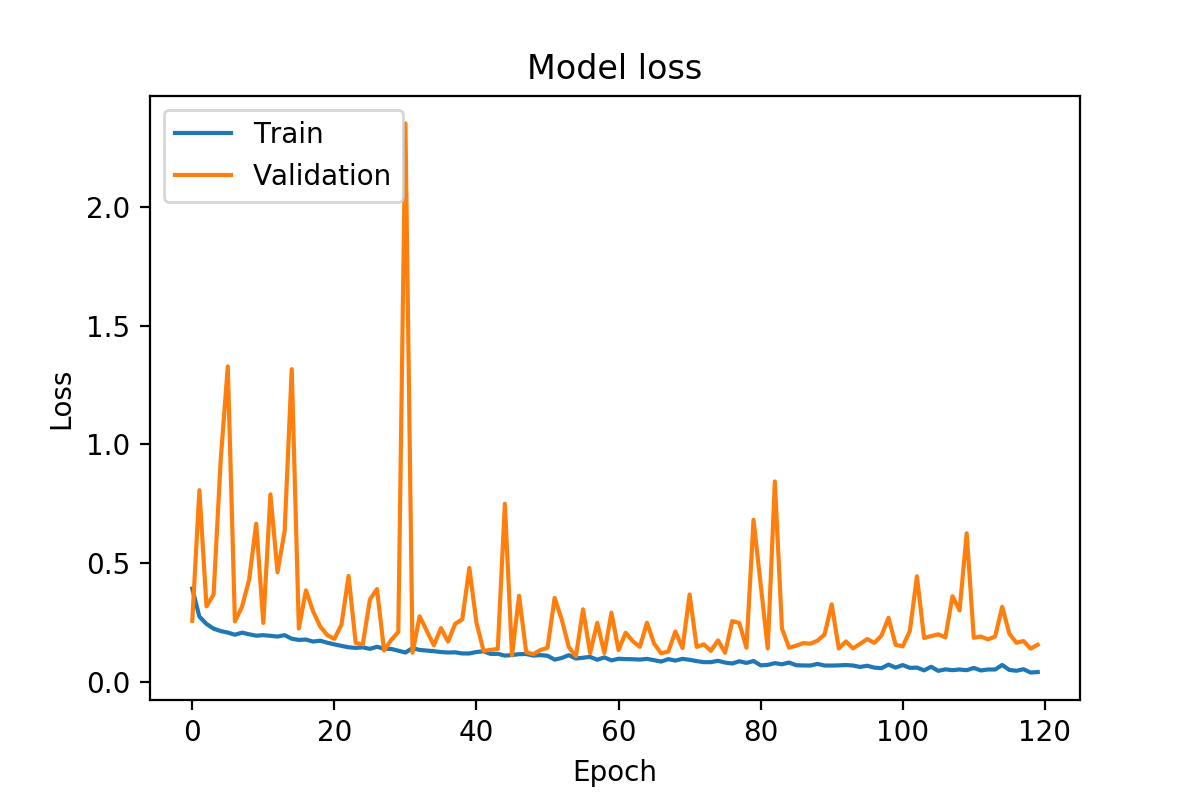
\includegraphics[width=0.9\linewidth]{mode_0_conv_1.png}
        \caption{Training plot for the ventilation mode 0}
    \end{figure}

    \begin{figure}[H]
        \centering
        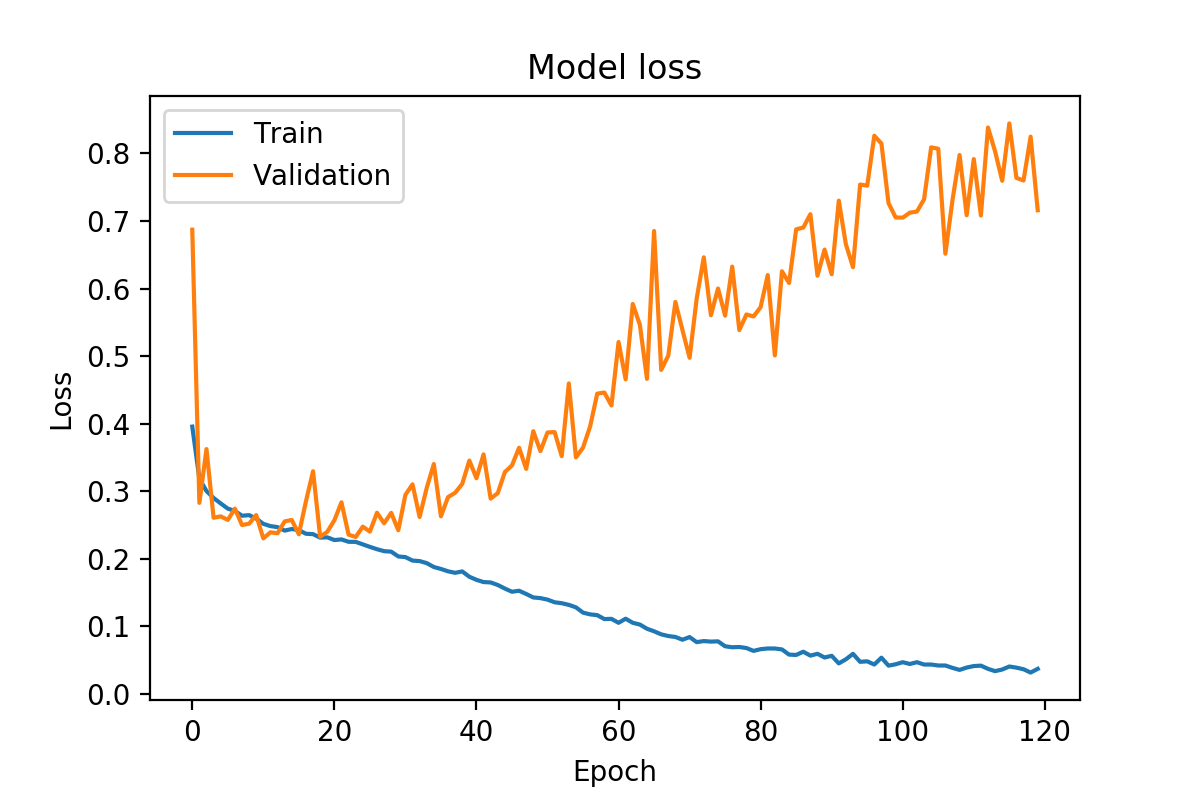
\includegraphics[width=0.9\linewidth]{mode_2_conv_1.png}
        \caption{Training plot for the ventilation mode 2}
    \end{figure}

    \begin{figure}[H]
        \centering
        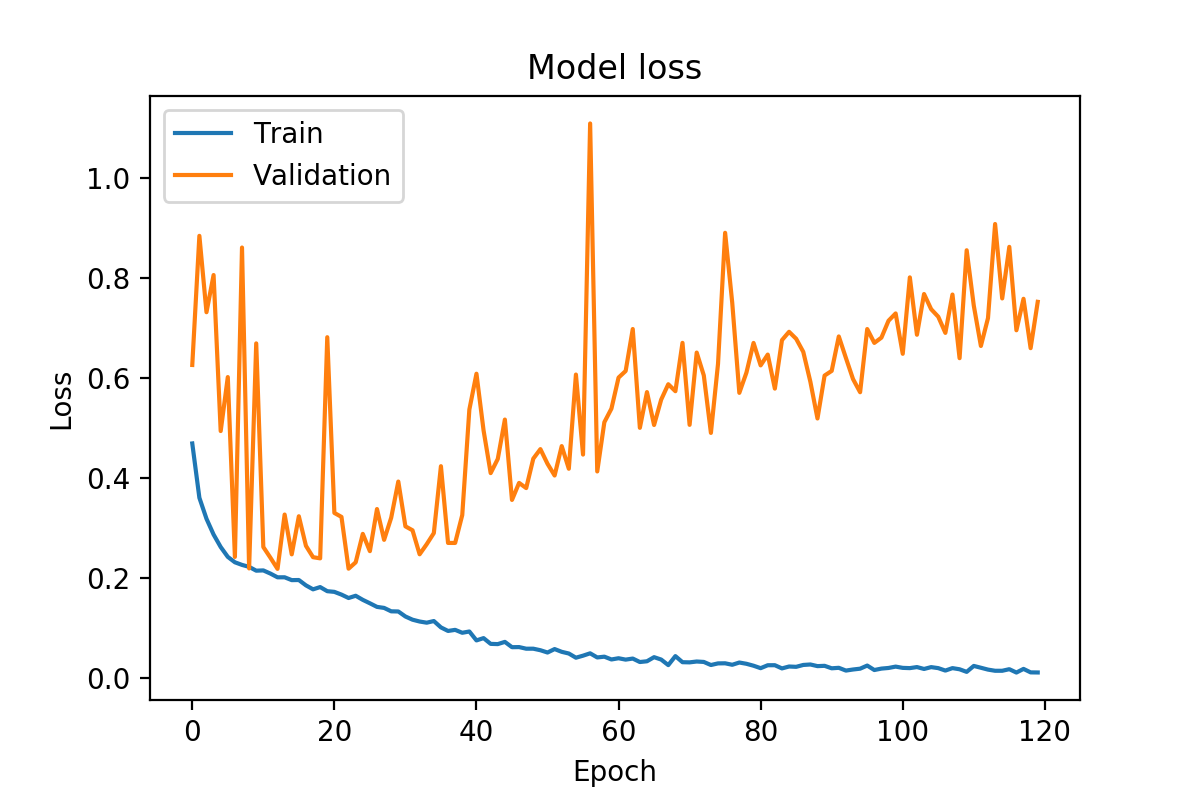
\includegraphics[width=0.9\linewidth]{mode_3_conv_1.png}
        \caption{Training plot for the ventilation mode 3}
    \end{figure}

    \begin{figure}[H]
        \centering
        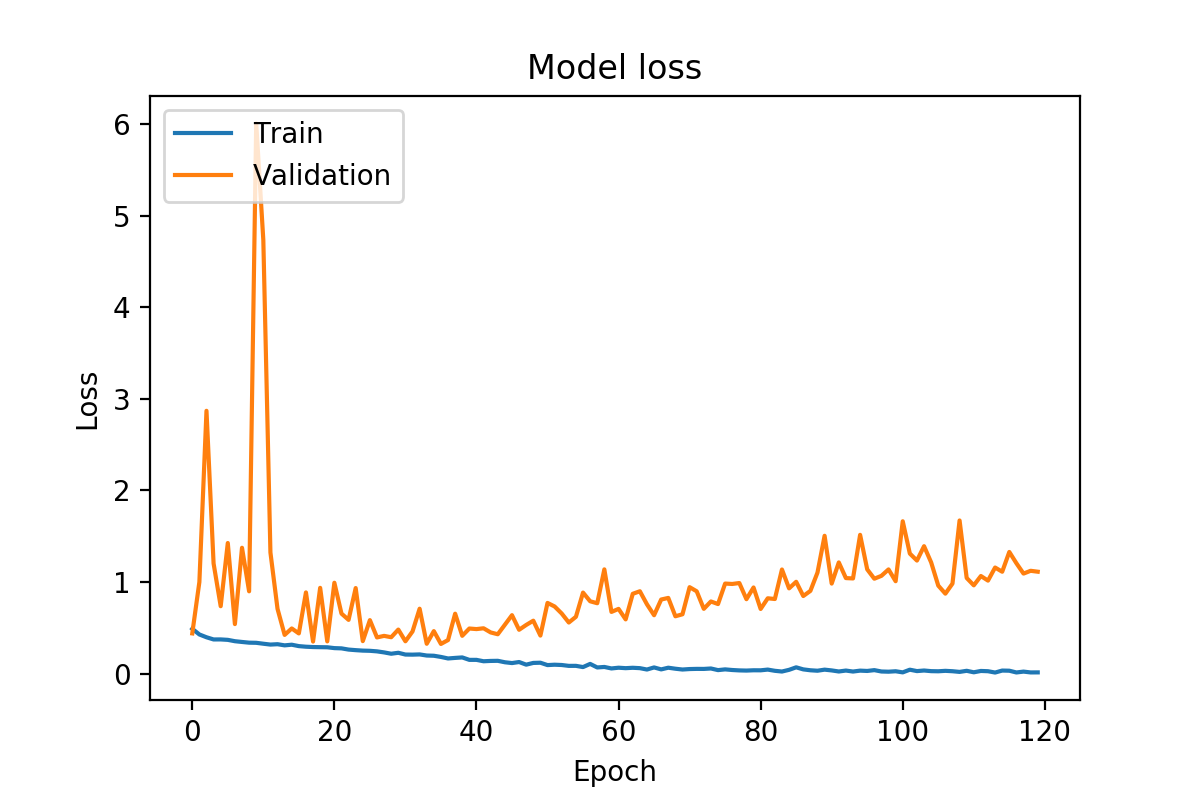
\includegraphics[width=0.9\linewidth]{mode_4_conv_1.png}
        \caption{Training plot for the ventilation mode 4}
    \end{figure}

It is clear that the first and last models converge very well with a small overfitting, while the second and third starts overfitting after few epochs. It has to be noticed that the latters have far more examples than the formers, and it is reasonable that after a number of epochs they start overfitting. Also, we selected a quite high number of epochs, 120; as a consequence, it is not so surprising that the models starts to overfit. However, since big differences are visible between plots and the network architecture is the same for each ventilation mode, the reason of this different behaviours could be redirected to properties which are inherent to the way in which the signals were collected.

For each model, after having measured the validation loss over 120 training epochs, we have set the number of training epochs to the number where the validation loss reached a minimum. Ultimately, we evaluated each model on its test set. The results are:

\begin{table}[H]
\begin{tabular}{l|l|l|l|l|}
\cline{2-5}
                                & MV 0 & MV 2 & MV 3 & MV 4 \\ \hline
\multicolumn{1}{|l|}{Precision} & 0.93 & 0.44 & 0.80 & 0.78 \\ \hline
\multicolumn{1}{|l|}{Recall}    & 0.99 & 0.88 & 0.98 & 0.91 \\ \hline
\multicolumn{1}{|l|}{F2\_score} & 0.98 & 0.74 & 0.93 & 0.88 \\ \hline
\end{tabular}
\end{table}

With respect to the chosen performance metrics, the $\mathcal{F}_2$ score, all the models except the second one performs quite well, especially the first. The second model, built on the data collected along the second ventilation mode, which we called MV 2, performs significantly worse than the others, even if for that specific mode the largest dataset was available.


\newpage

\section{Conclusion}

The convolutional neural network has produced rather good results on all but the second ventilation mode. We think this results can be a good starting point for further investigations. A point to be inspected is what induces the performance differences between the ventilation modes, but we suspect a domain knowledge on mechanical ventilation would be required for a satisfactory explanation.

Also, it would be interesting to look for more sophisticated architectures to additionally increase the accuracy in spotting those breaths containing asychronies. An example is an architecture called \textit{Transformer}, which makes use of the \textit{attention mechanism} and, if well tuned, would probably reach better performances without a significant variation of the computational cost.

The following, more subtle, step would be to predict in runtime the emergence of asynchronies in a signal. For this purpouse, \textit{sequence-to-sequence} techniques will be needed.


\newpage

\section*{Ringraziamenti}

Dedico questo lavoro di tesi alla mia famiglia, senza il supporto della quale non avrei potuto intraprendere questo percorso di crescita. In particolare, ai miei genitori, per la pazienza e la fiducia con cui mi hanno nutrito quotidianamente; a Chiara e Christian, per essere cresciuti con me; a mia nonna, per la non superata dolcezza; a mio nonno, per essere stato il primo a farmi alzare gli occhi verso le stelle.

Ringrazio infinitamente il mio relatore, Luca, senza il quale non solo questo lavoro di tesi, ma una grande fetta del mio entusiasmo verso la Computational Intelligence, non esisterebbe. Le conversazioni felicemente informali portate avanti negli ultimi tempi sono state il motore del mio interesse verso un percorso che trascende questo lavoro in sé, e ciò è senza prezzo.

Al mio co-relatore, il prof. Marco Budinich, devo la scintilla iniziale che ha acceso il mio interesse verso le reti neurali. Se non avessi seguito il suo corso di \textit{Introduzione alle Reti Neurali}, non avrei compiuto molte delle scelte che oggi mi rendono soddisfatto di ciò che faccio.

Un grande grazie è per Michele Rispoli, per avermi ispirato con quel fatidico incontro fuori dal supermercato, spesa in mano, in cui mi raccontò del suo lavoro di tesi, e avermi fornito una indispensabile e solida base su cui lavorare.

Ho la fortuna di conoscere molte persone più notevoli e preparate di me, con le quali porto avanti conversazioni che non smettono di riforgiarmi con nuovi spunti, conoscenze ed interessi. Di queste, desidero ringraziare Salvatore Miceli, Emanuele Ballarin e Francesco Zuppichini, per le frequenti corrispondenze a tema machine learning, le quali non smettono di divertirmi ed arricchirmi; Alessia Menichetti, per avermi accompagnato negli ultimi tre anni e a cui, ne sono certo, devo la grandezza delle mie ambizioni e la sicurezza con cui scelgo di inseguirle; Fabrizio Bigotti, per essere stato e continuare ad essere per me un grande mentore e grandissimo amico.

Infine, grazie a Matei Tiloiu, un amico storico con cui ho sempre condiviso l'entusiasmo per ciò che è nuovo, diverso e ancora incompreso.








\newpage

\nocite{*}

\bibliography{references}
\bibliographystyle{plain}


\newpage

\appendix
\section{Architecture diagram}

\begin{figure}[H]
    \centering
    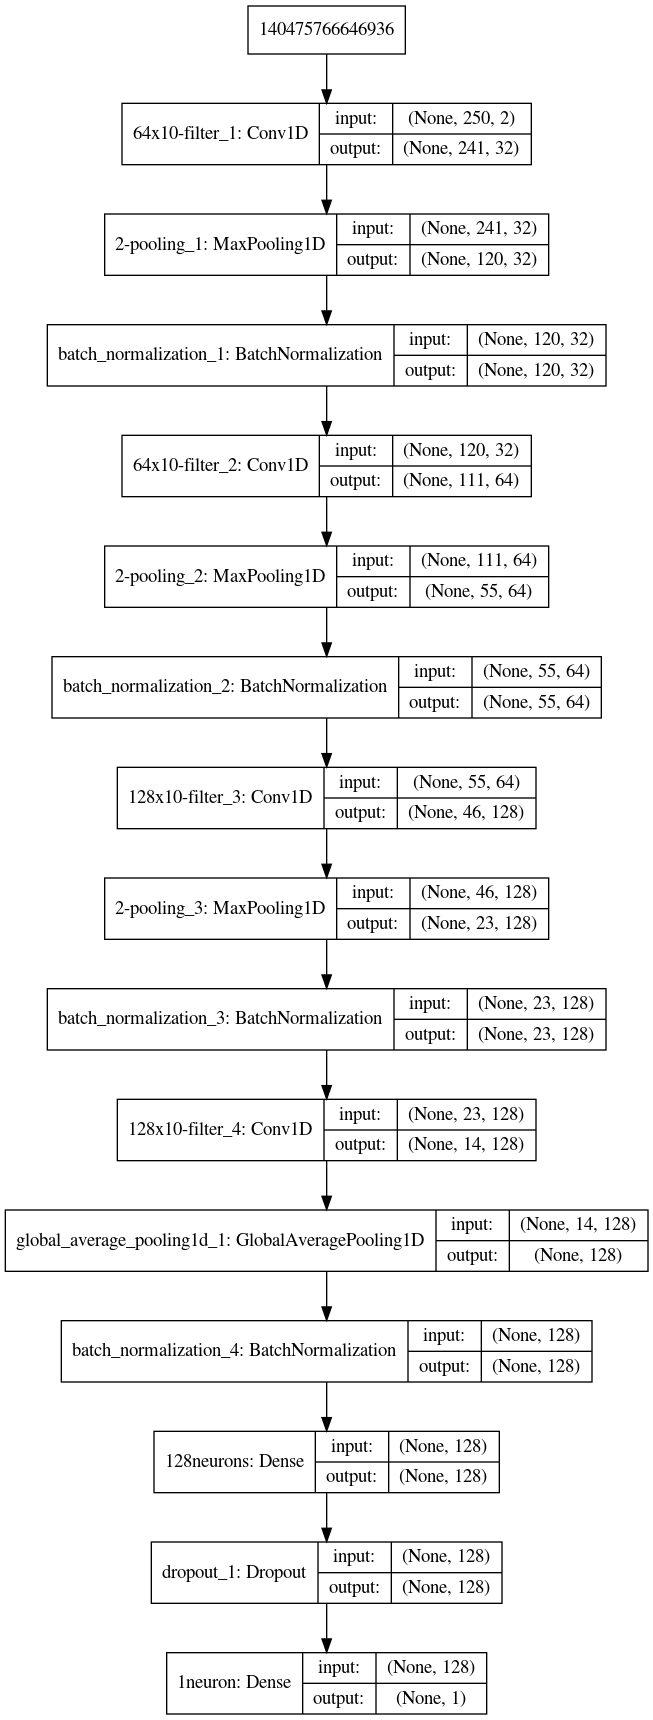
\includegraphics[width=0.50\linewidth]{model_mode0.png}
    \caption{Architecture diagram}
\end{figure}





\end{document}

